\documentclass[11pt]{article}
\usepackage{geometry}
\usepackage{graphicx}
\usepackage{epstopdf}
\usepackage{listings}
\usepackage{float}
\usepackage{csvsimple}
\usepackage{wrapfig}
\usepackage{longtable}

\begin{document}
\section{1/24/16}
\subsection{Permutation testing}
In order to test how the algorithm returns the permutation results, I set up sample matrices using \verb|create_toy.m| and recorded the distance between the result returned by the algorithm (\verb|eig_perm|) and that of the actual input data (\verb|ss|).

\lstset{language=Matlab, caption=Compare Permutations}
\begin{lstlisting}[frame=single]
rois = 33;
noise_mag = 0;
trace_type = 'sines';
shift = 10;
y = zeros(1,100);
for i = 1:length(y)
	[Z, ss] = create_toy(trace_type, 'rois', rois, ...
		'noisemag', noise_mag, ...
		'shift', shift);
	[eig_phases,eig_perm,slm,evals] = cyclic_analysis(Z);
	y(i) = cyclic_distance(ss,eig_perm);
end
plot(y)
\end{lstlisting}

The function \verb|create_toy| produces a set of \verb|rois| identical sine waves randomly spread over a \verb|shift| time step period (i.e., each copy of the trace is shifted along the x axis so that all copies are within \verb|shift| time steps of each other). The variable \verb|ss| shows the ordering of the traces produced. Using the setting above, for example, a data set like that in on the left of Figure 1 is produced. The figure on the right shows that the algorithm returns the identical permutation each time.
\begin{figure}
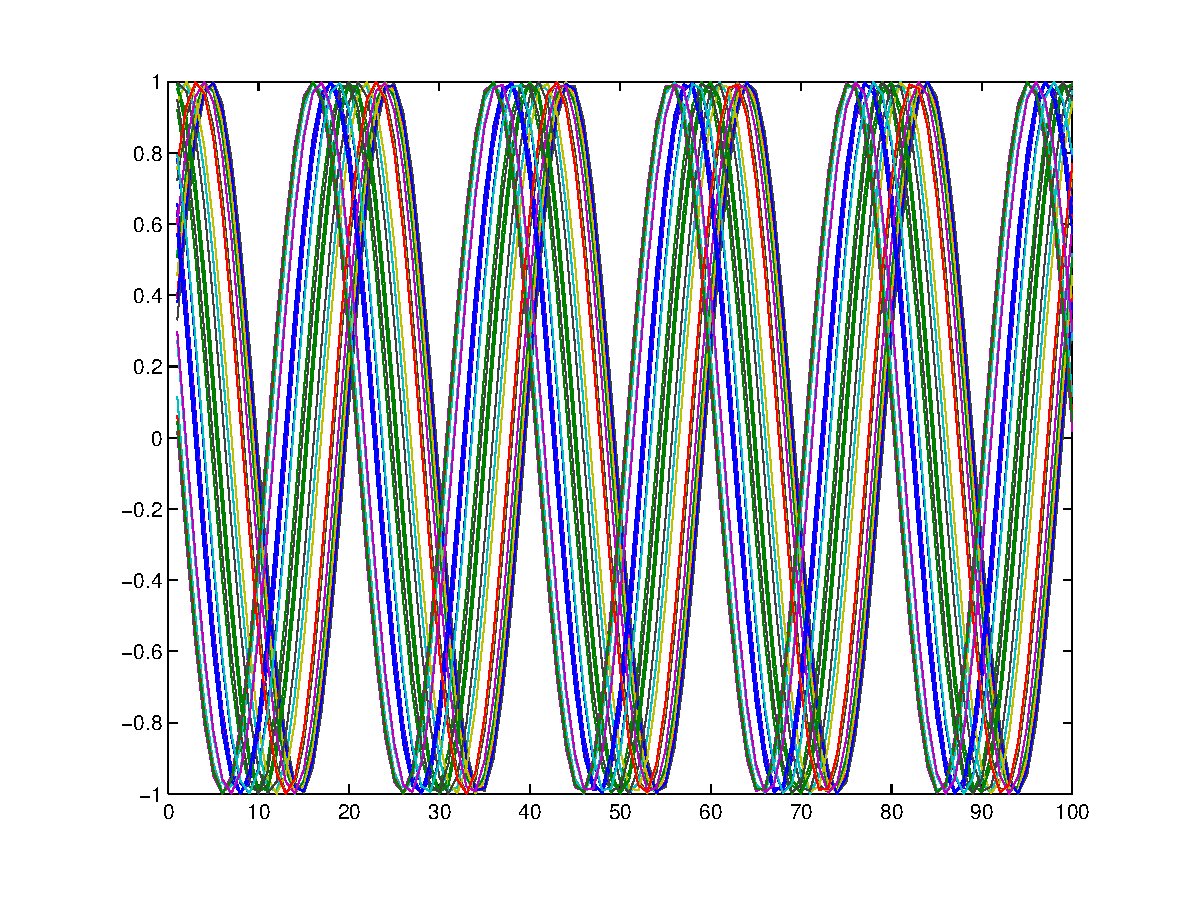
\includegraphics[width=.45\textwidth]{pictures/1_24_16/sine_toy.eps}
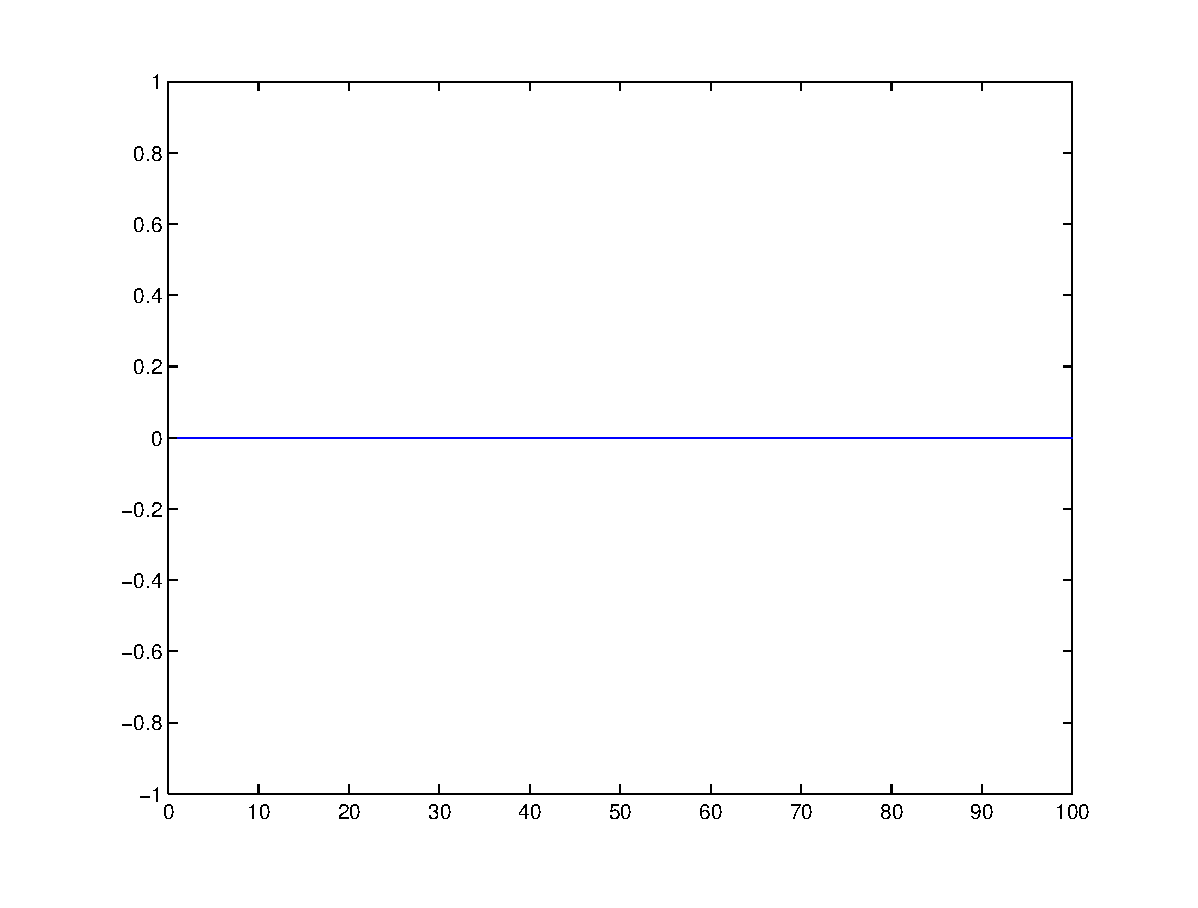
\includegraphics[width=.45\textwidth]{pictures/1_24_16/sine_cpsn_noNoise.eps}
\caption{Left: Sample data created from sine waves shifted randomly at most 10 time steps apart (no added noise). Right: Comparison of the permutation returned by the algorithm with that of the actual data set for 100 separately generated data sets.}
\end{figure}
The distance is measured using \verb|cyclic_distance(V1,V2)| which simply counts the how many steps V2 is from V1 (let V1 be (1:5), then [2,1,3,4,5] is a distance of 1 from V1 and [2,3,4,5,1] is a distance of 5 from V1.) This doesn't really count "cyclic distance" but works for this application since we would like to see if we are picking up the correct starting point and cycling in the right direction. 
Increasing \verb|shift| to 18 (the period for the sine wave is 20) starts to mess up the permutation since the algorithm can't determine the proper starting point.
\begin{figure}[H]
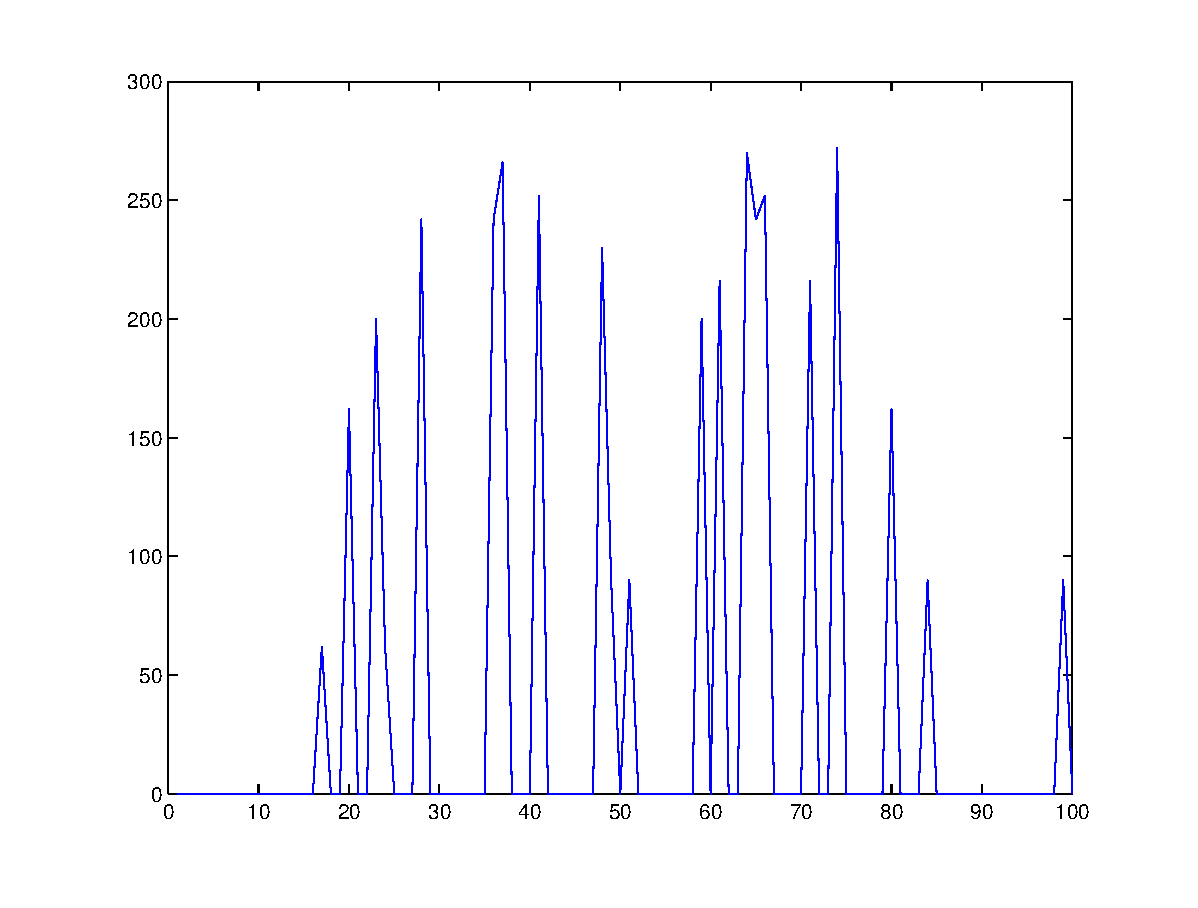
\includegraphics[width=.45\textwidth]{pictures/1_24_16/sine_cpsn_shift18.eps}
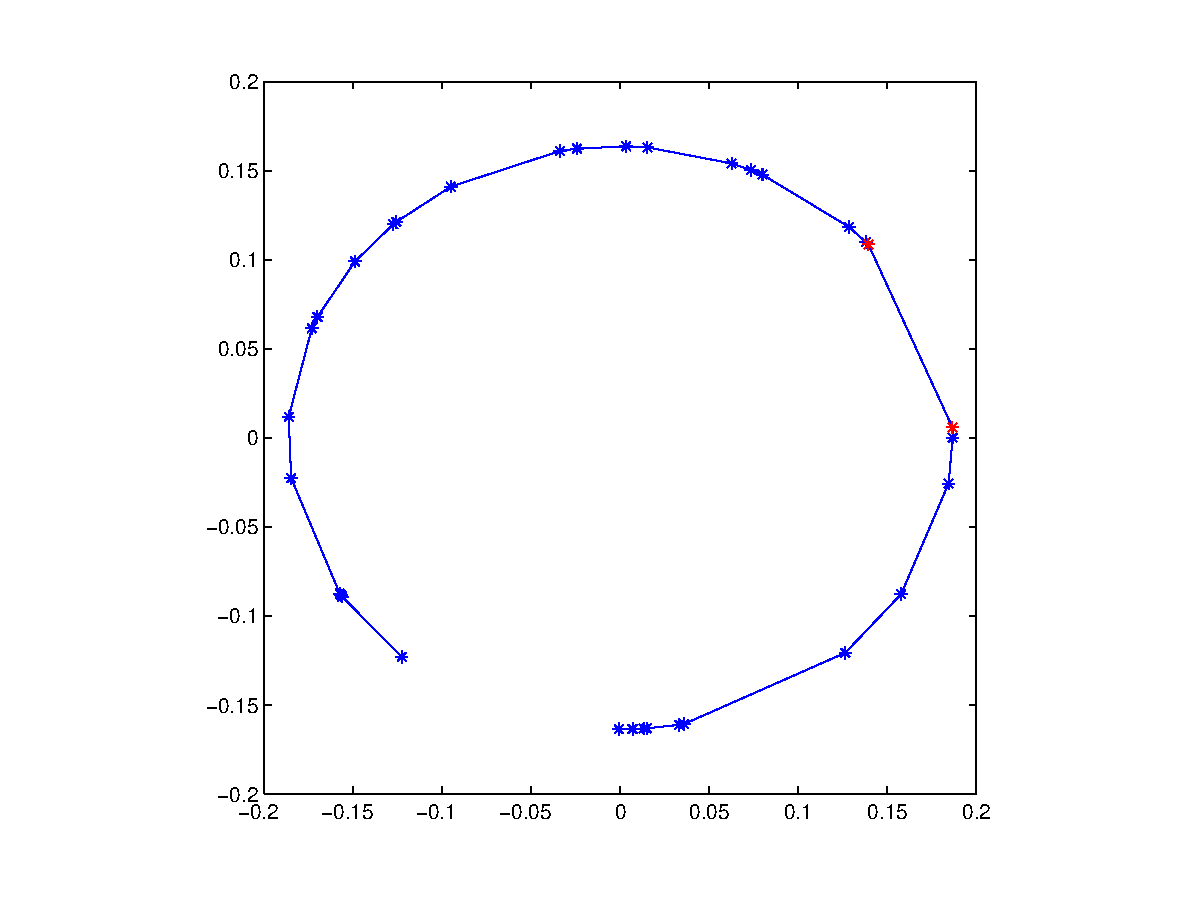
\includegraphics[width=.45\textwidth]{pictures/1_24_16/phases_shift18.eps}
\caption{Left: Algorithm performance when \texttt shift=18. Right: Plot of phases for a permutation which the algorithm had shifted by 11 places (distance = 242). The red asterisks highlight the 11th and 12th points in the cycle.}  
\end{figure}
The algorithm determines the starting point by finding the largest gap between points in the phase plot (greatest difference in angle). Once the phases are too spread out, the largest gap can easily be between a pair of middle points. Note, however, that still the algorithm cycles in the correct direction in each case. 


\section{Listings}
\lstset{language=Matlab, caption=cyclic\_distance}
\begin{lstlisting}[frame=single]
function [dist] = cyclic_distance(V1, V2)
[~, ss] = sort([V1(:), V2(:)]);
dist = sum(abs(diff(ss,1,2)))/2;
\end{lstlisting}

\subsection{Movies}
\subsubsection{Data Treatment}
In the original data set, there are gaps in the data for some genres and not all genres began at the same time so some initial data treatment was required. First, years in which there were gaps in the data were inpainted using linear interpolation. Next, the genre counts were taken on a log scale to account for the fact that movie production has grown exponentially. Finally, only years in which genres had data points were considered (1916-2015). The film-noir genre had to be excluded since the production years were so limited.
The following table shows the results of \verb|analyze_cyclicity| on the movie data (processed as described above). 
\begin{figure}[H]
\begin{minipage}{.3\textwidth}
\csvautotabular{tables/genre_results.txt}
\end{minipage}
\hfill
\begin{minipage}{.65\textwidth}
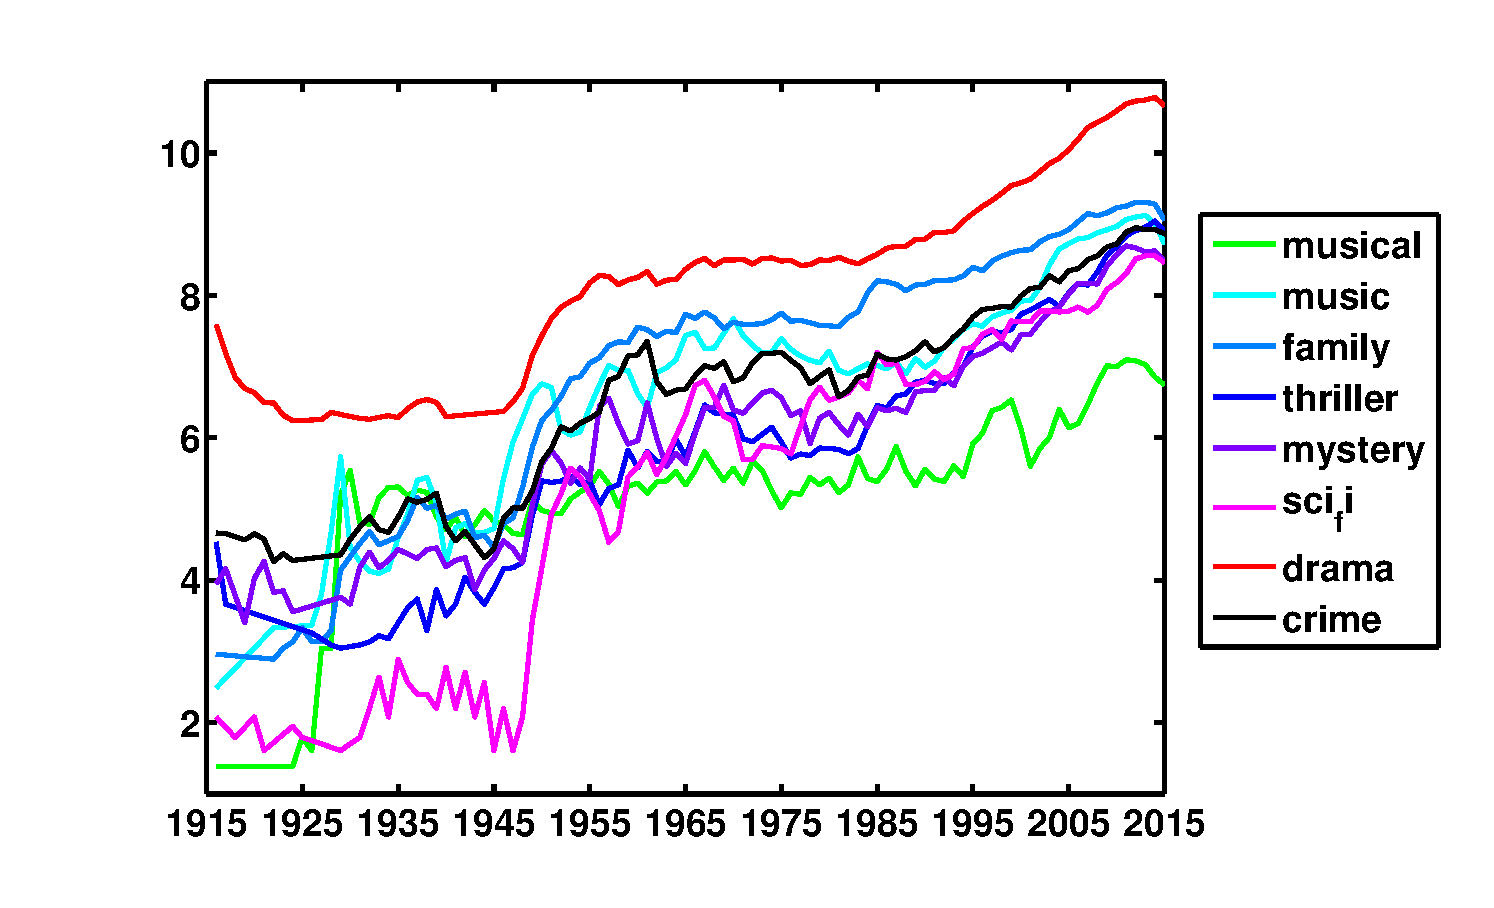
\includegraphics[width=\textwidth]{pictures/movie_data_all_yrs.eps}
\caption{Traces from the first eight genres.}
\end{minipage}
\end{figure}
\begin{figure}[H]
\centering
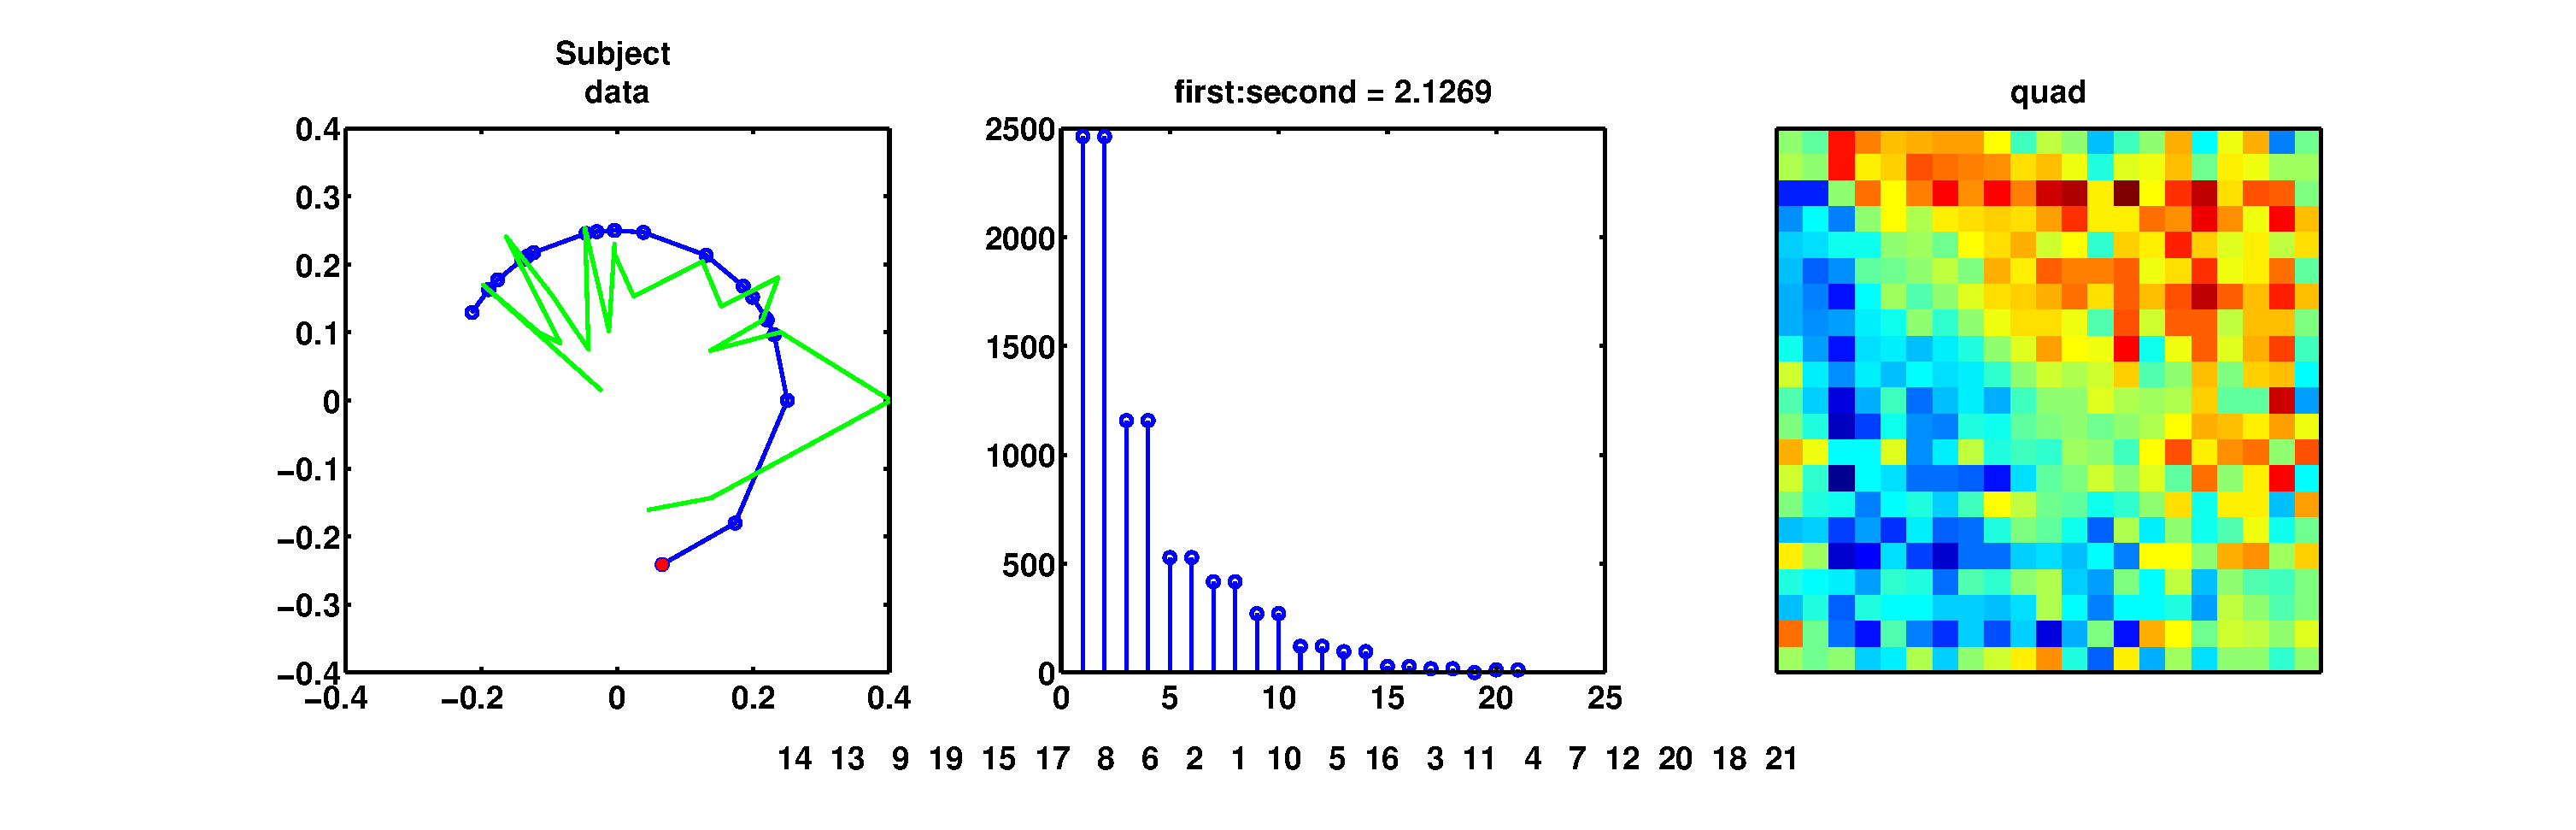
\includegraphics[trim= 130 0 130 0, clip, width=\textwidth]{pictures/movie_data_QC.eps}
\caption{Cyclicity results using quadratic variation normalization}
\end{figure}
Note that the Musicals and Music genres look very similar to each other, but dissimilar to everything else and show a drastic jump around 1925. Since this is such a long time ago, it seemed worth considering more recent trends in the data.
\begin{figure}[H]
\begin{minipage}{.3\textwidth}
\csvautotabular{../Movies/Recent_data/Results/genre_results_table.txt}
\end{minipage}
\hfill
\begin{minipage}{.6\textwidth}
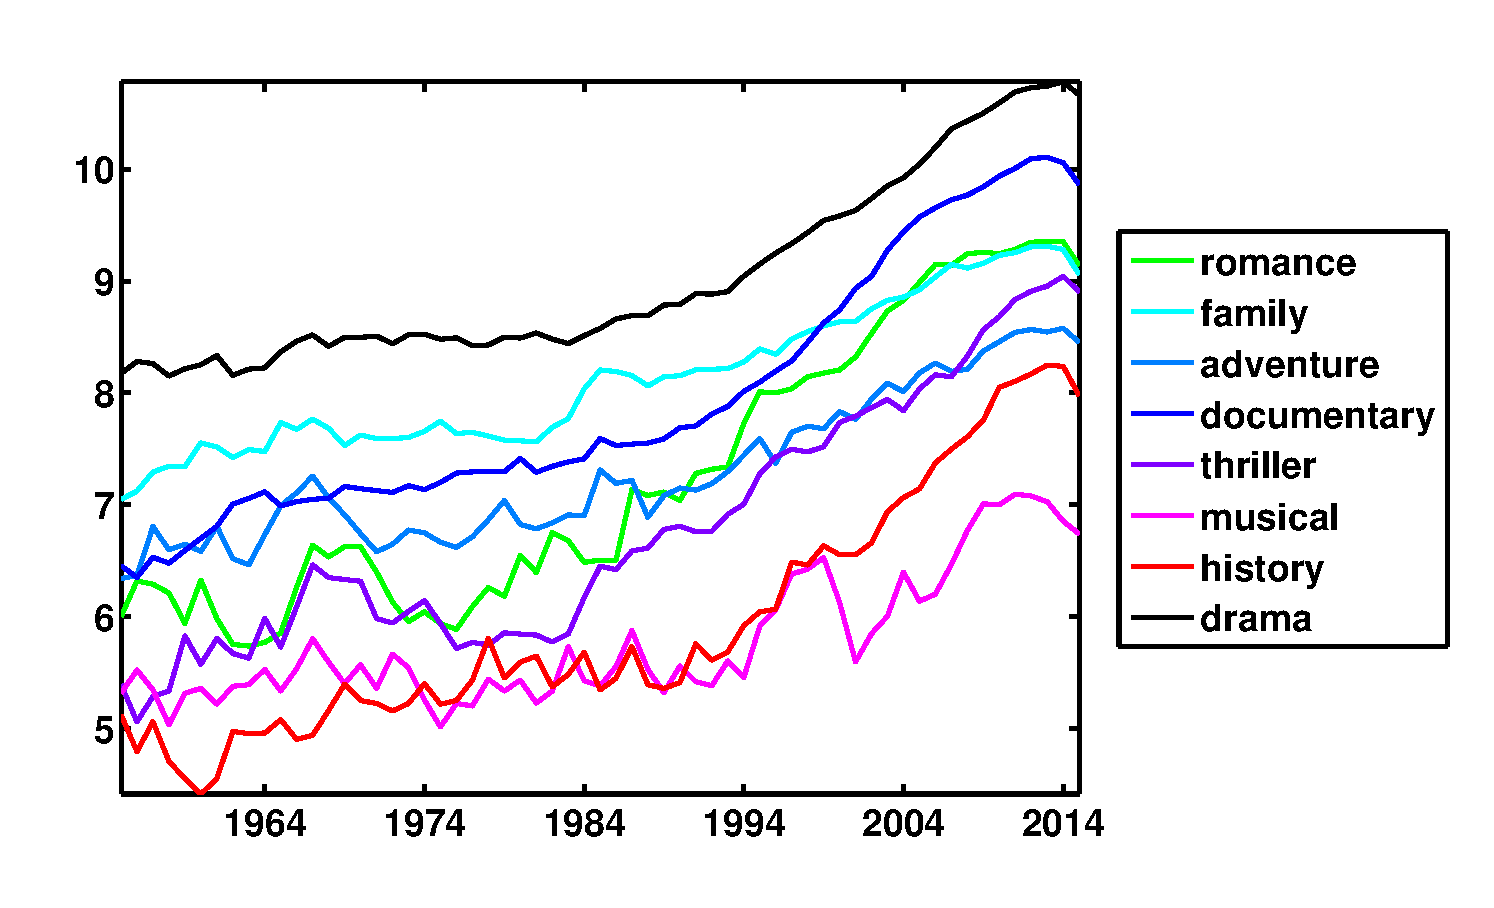
\includegraphics[width=\textwidth]{pictures/movie_data_1955-2015.eps}
\caption{Traces from the first eight genres using only years 1955-2015 in the cyclicity calculation.}
\end{minipage}
\end{figure}
\begin{figure}[H]
\centering
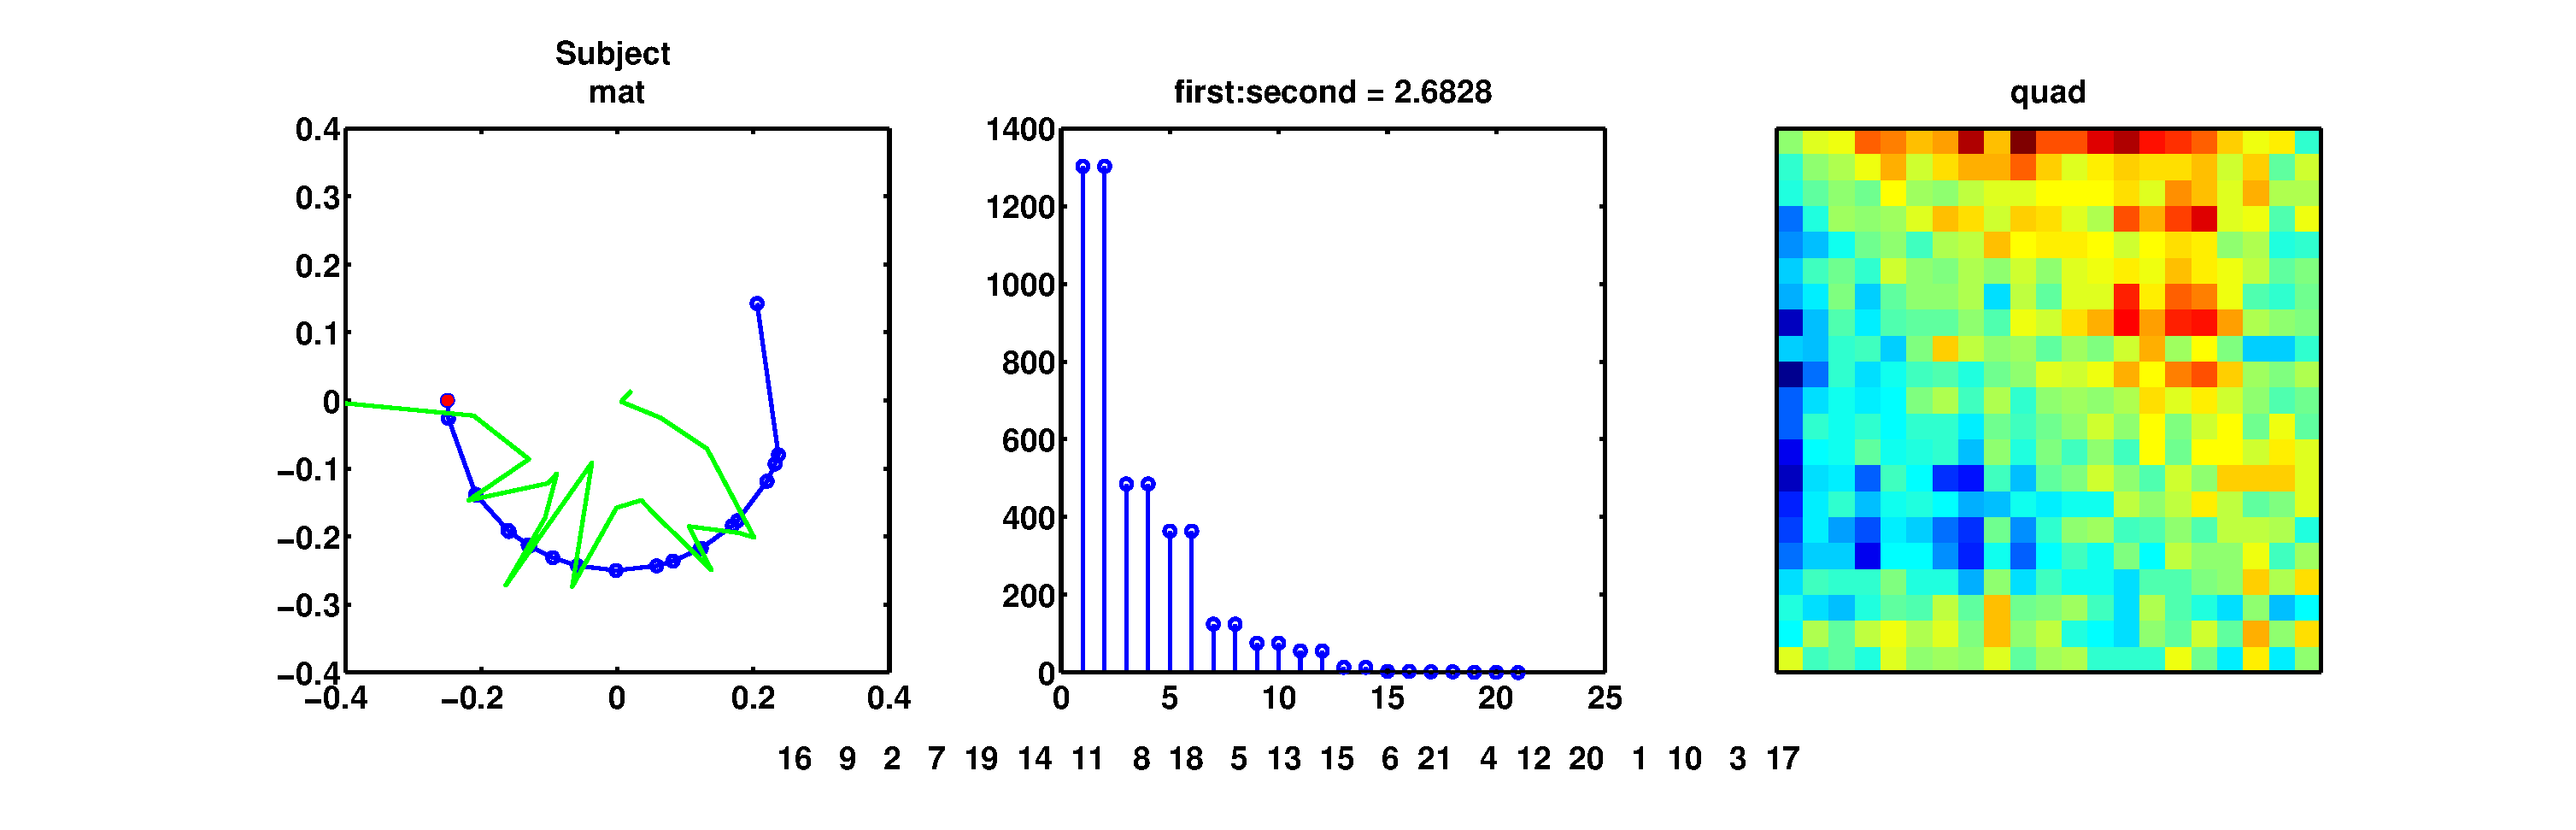
\includegraphics[trim= 130 0 130 0, clip, width=\textwidth]{pictures/movie_data_1955-2015_QC.eps}
\caption{Cyclicity results from 1955-2015 movie data using quadratic variation normalization}
\end{figure}

\section{2/2/16}
\subsection{Movie trends with words counts from New York Times}

We added some word trends to the movie data, taking search counts for selected words on the New York Times website. The search was filtered by year so that we could get word counts for each year that we have movie data for (1916-2015). Word counts were pulled using \verb|times_scrape.py| and looping through the years in a bash script (see scraping folder in Movies). The words searched were searched

\begin{center}
\begin{tabular}{lllll}
crisis&
terror&
war&
attack&
expansion\\
growth&
invasion&
prosperity&
shooting&
\end{tabular}
\end{center}

and the following results obtained:

\begin{figure}[H]
\centering
\begin{minipage}{.25\textwidth}
\csvautolongtable{tables/movie_word_perm_results_p1.txt}
\end{minipage}
\begin{minipage}{.25\textwidth}
\csvautolongtable{tables/movie_word_perm_results_p2.txt}
\end{minipage}
\begin{minipage}{.25\textwidth}
\csvautolongtable{tables/movie_word_perm_results_p3.txt}
\end{minipage}
\caption{Resulting permutation from full movie and word analysis}
\end{figure}

\begin{figure}[H]
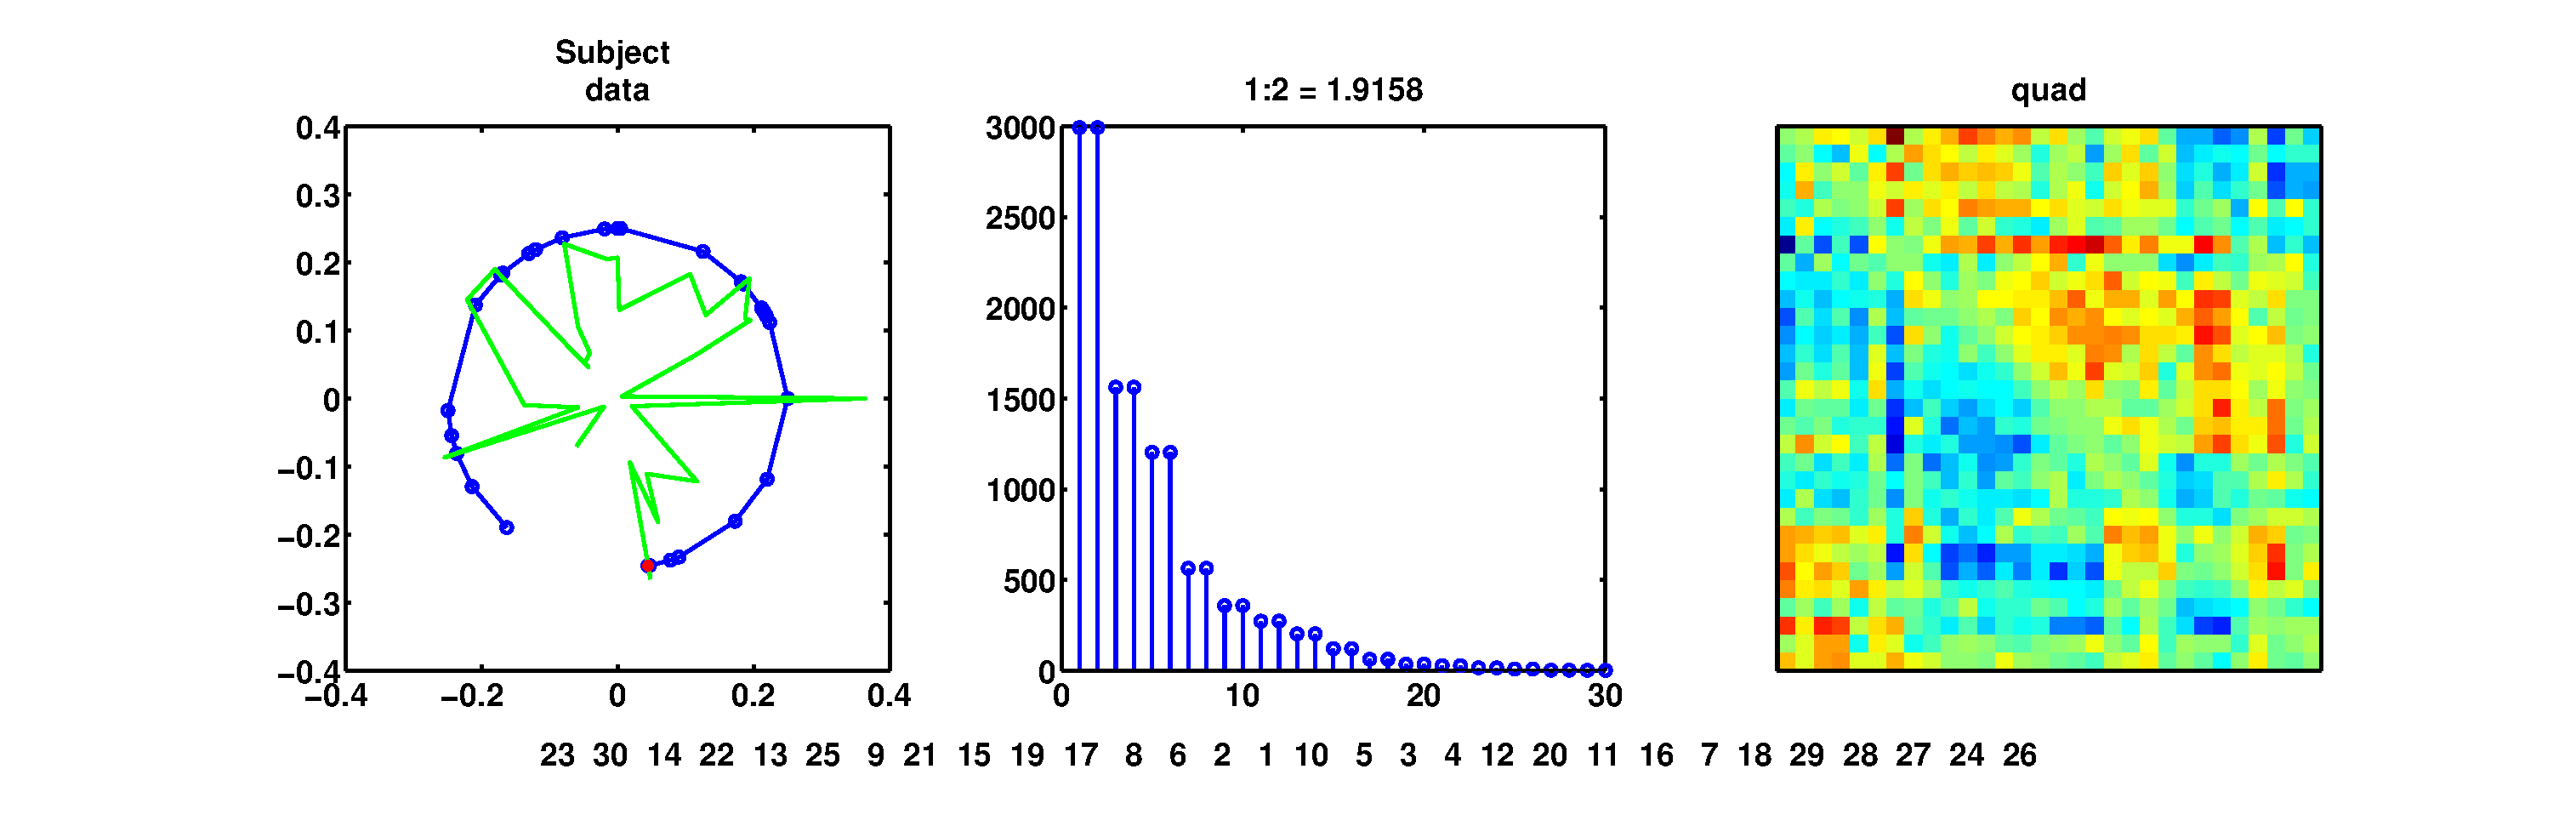
\includegraphics[trim = 150 0 130 0, clip, width=\textwidth]{pictures/movie_word_all.eps}
\caption{Results of full movie and word analysis}
\end{figure}

\subsection{Refining Movie-word results}
Next, we wish to consider smaller subsets of traces using the magnitude of the phase associated with a trace as an indicator of agreement with a particular ordering. For each set of figures, \verb|p| indicates which eigenvector was used to generate the ordering , \verb|n| indicates how many categories were used in the smaller group analysis and \verb|group| is which subset of the full set. So, for example, if \verb|p=1|, \verb|n=8|, \verb|group=1| then the first eigenvector was used to generate an ordering of full set of categories and then the eight categories with the highest magnitude of associated phase vector were pulled out and reanalyzed using the cyclicity algorithm to yield the ordering shown in the legend. If \verb|group=2| the group 1 categories were pulled out of the original data set and then the same procedure was followed, ordering the categories associated with the top eight phases of this smaller subset. When \verb|p=2|, the second eigenvector is used in the cyclicity algorithm to generate the ordering.

\begin{figure}[H]
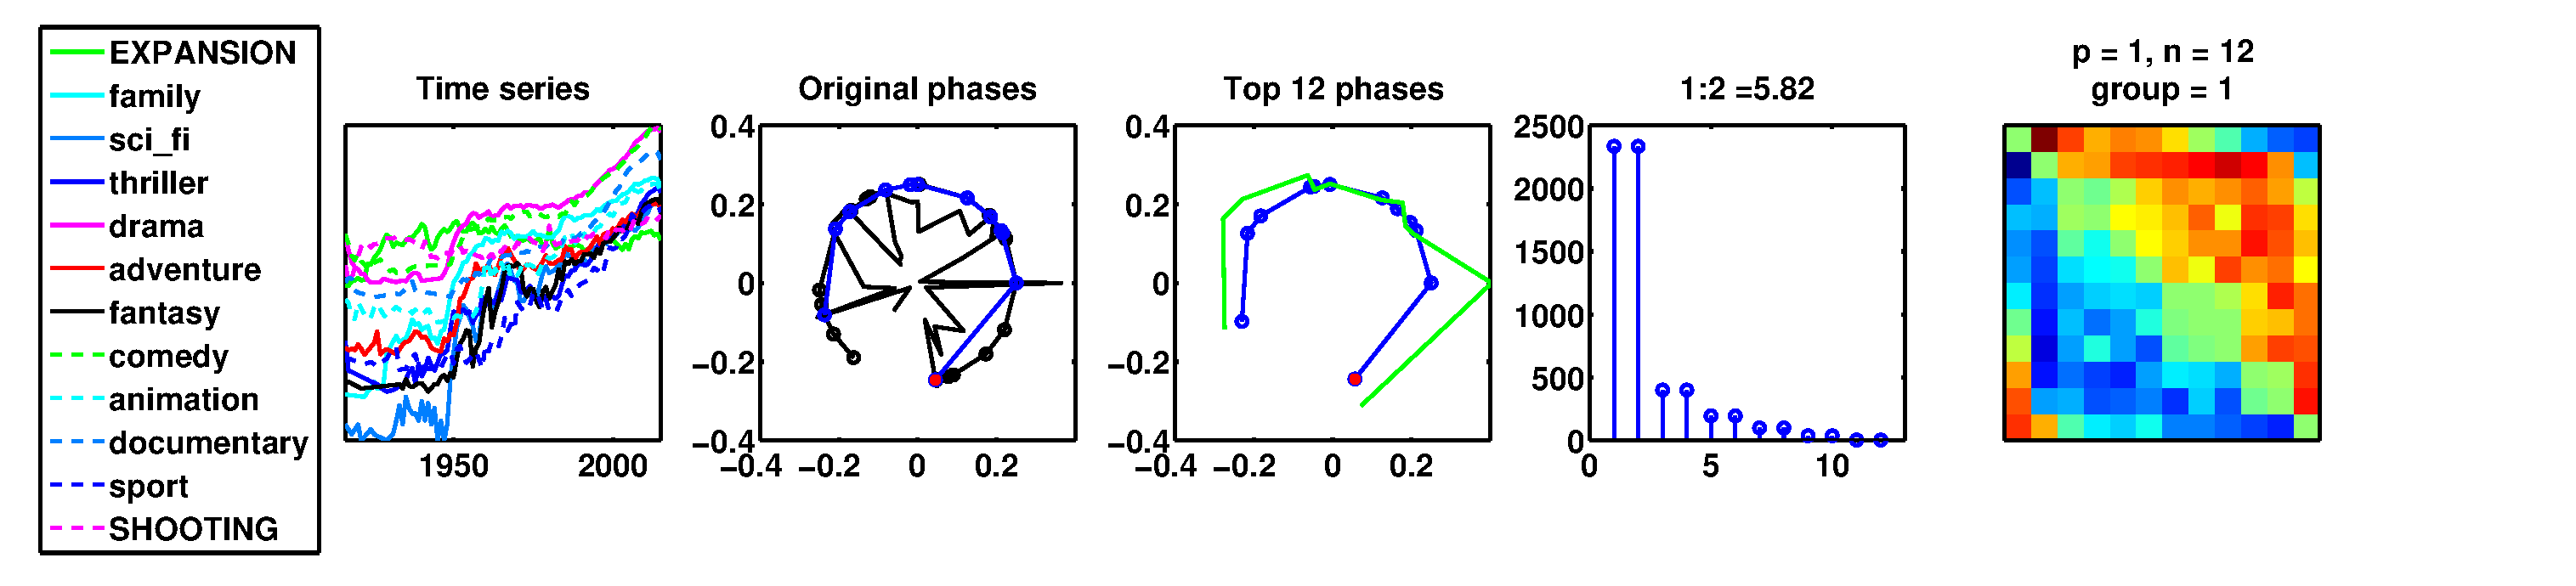
\includegraphics[trim = 0 0 130 0, clip, width=\textwidth]{pictures/_p1_n12_gp1.eps}
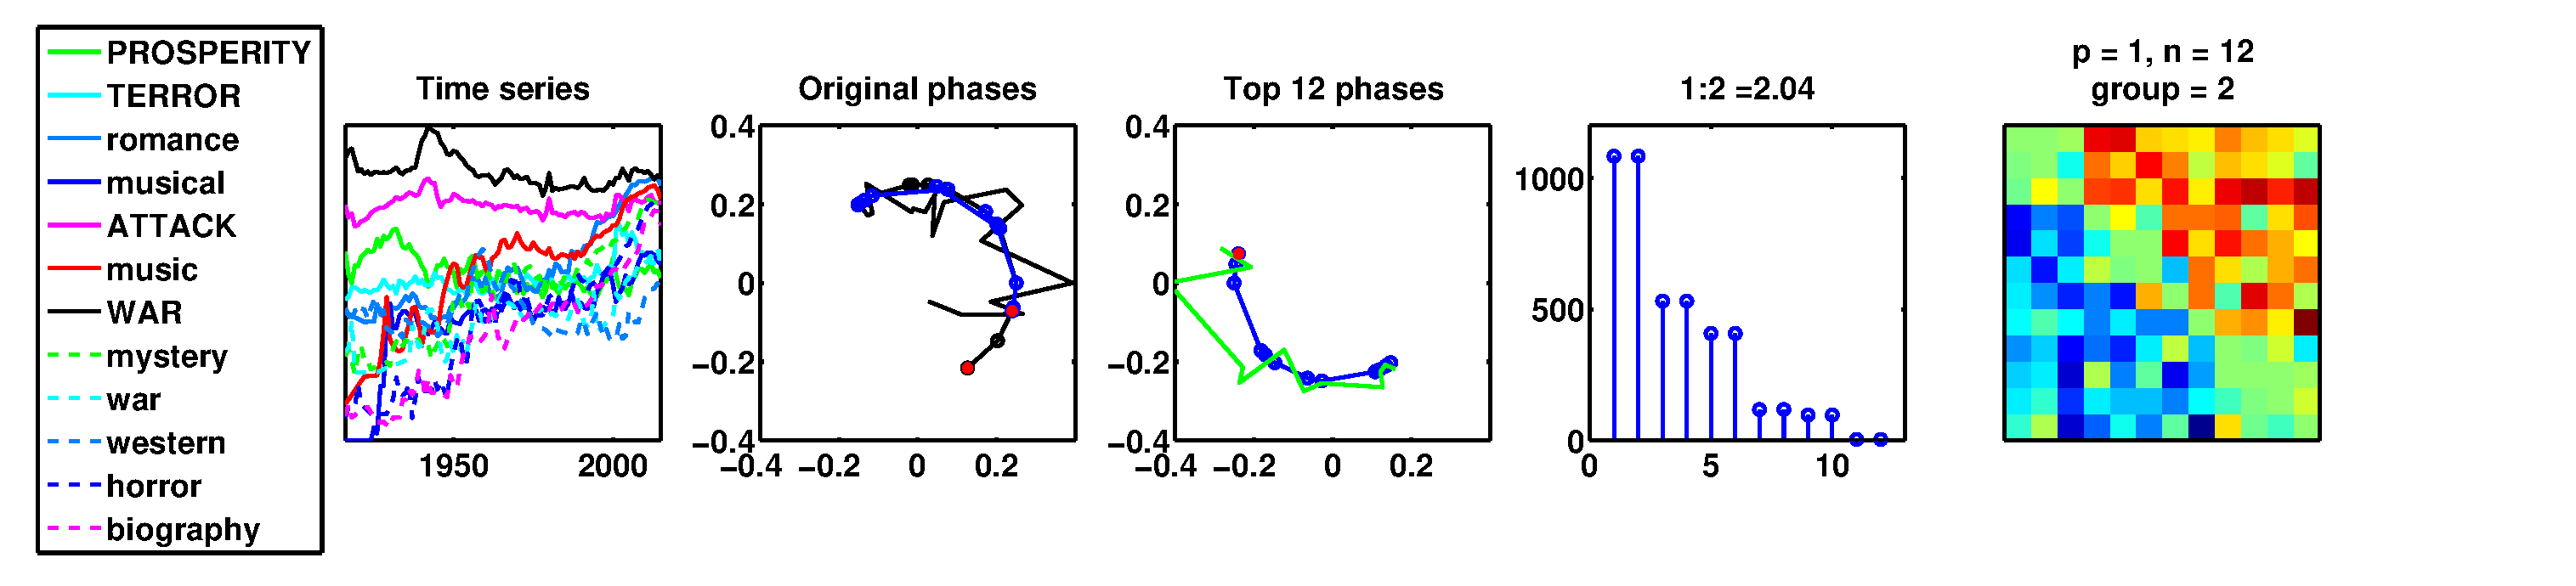
\includegraphics[trim = 0 0 130 0, clip, width=\textwidth]{pictures/_p1_n12_gp2.eps}
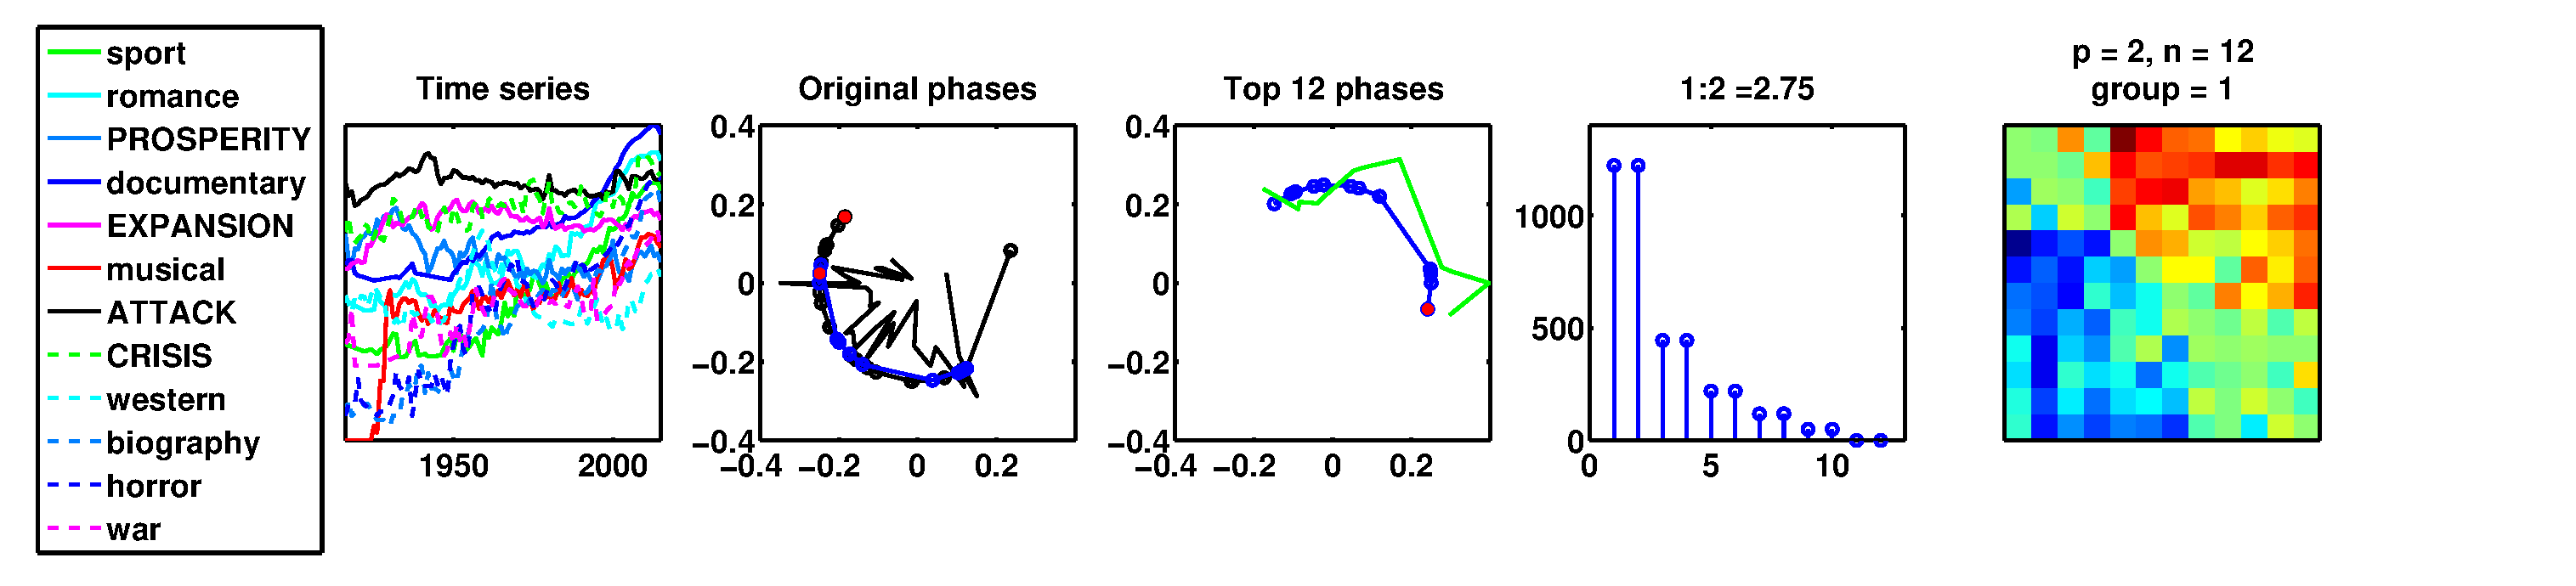
\includegraphics[trim = 0 0 130 0, clip, width=\textwidth]{pictures/_p2_n12_gp1.eps}
\caption{Results with n=12.}
\end{figure}

\begin{figure}[H]
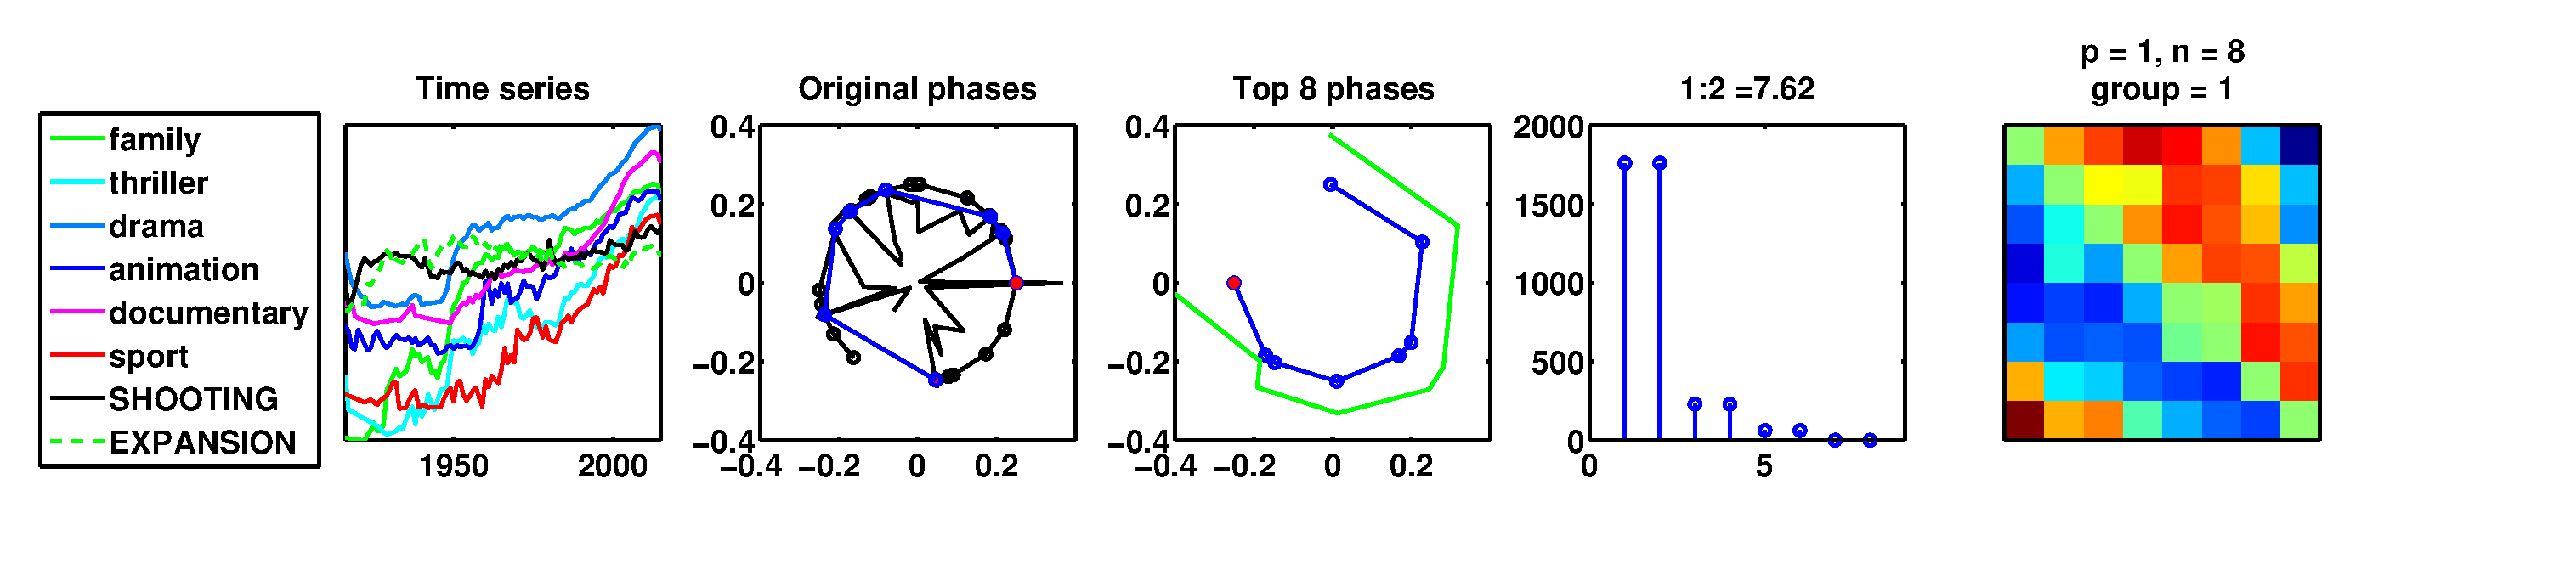
\includegraphics[trim = 0 0 130 0, clip, width=\textwidth]{pictures/_p1_n8_gp1.eps}
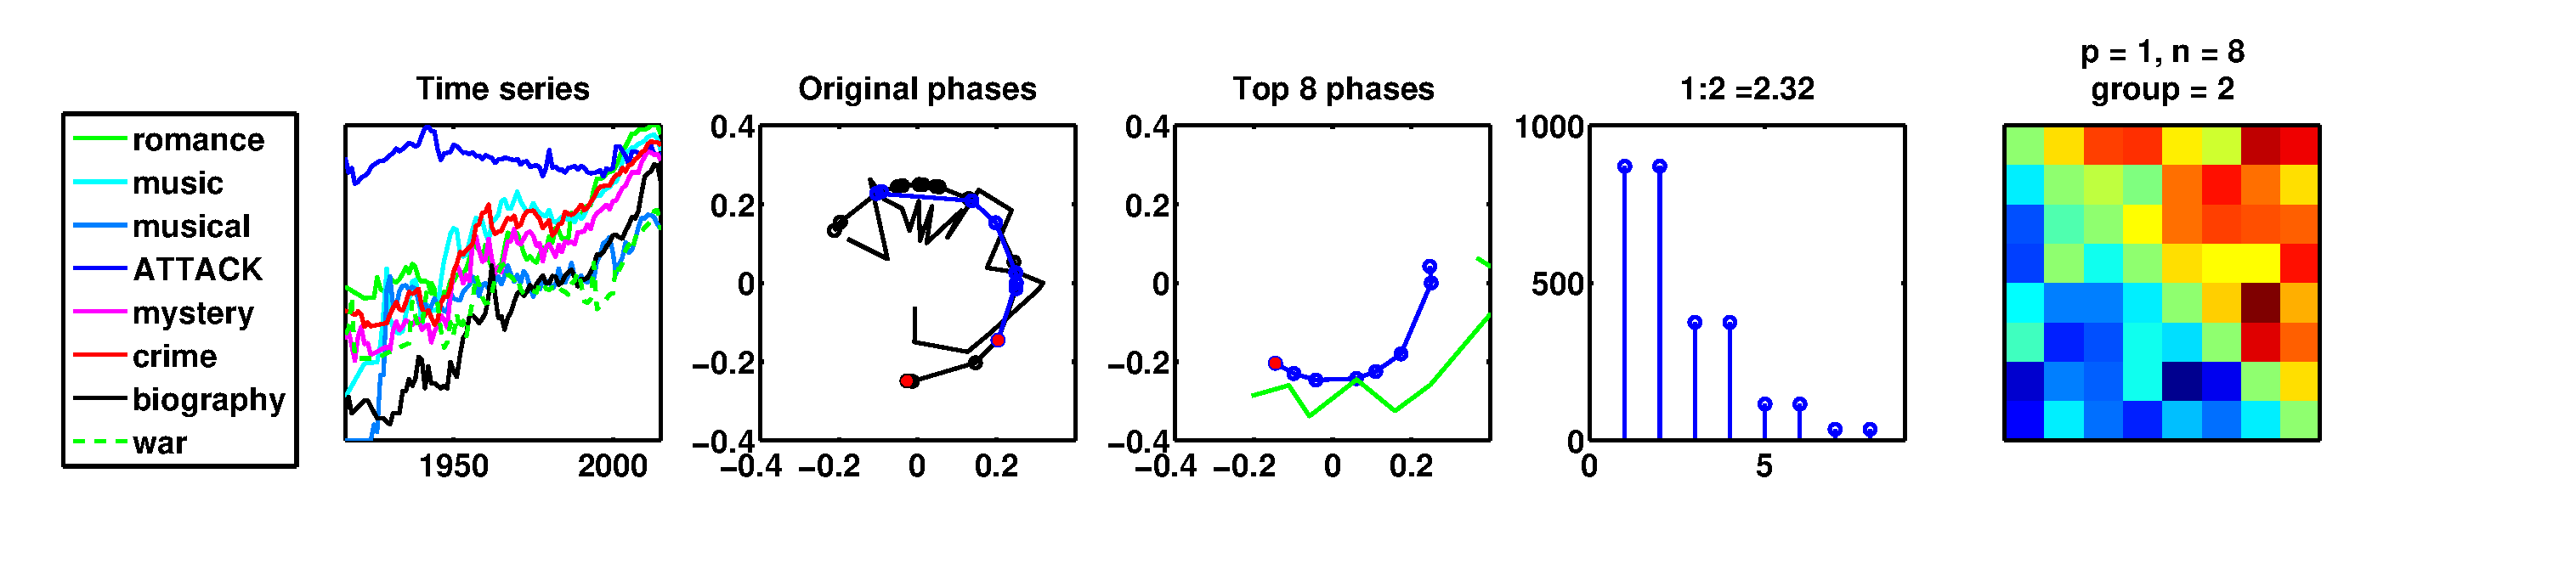
\includegraphics[trim = 0 0 130 0, clip, width=\textwidth]{pictures/_p1_n8_gp2.eps}
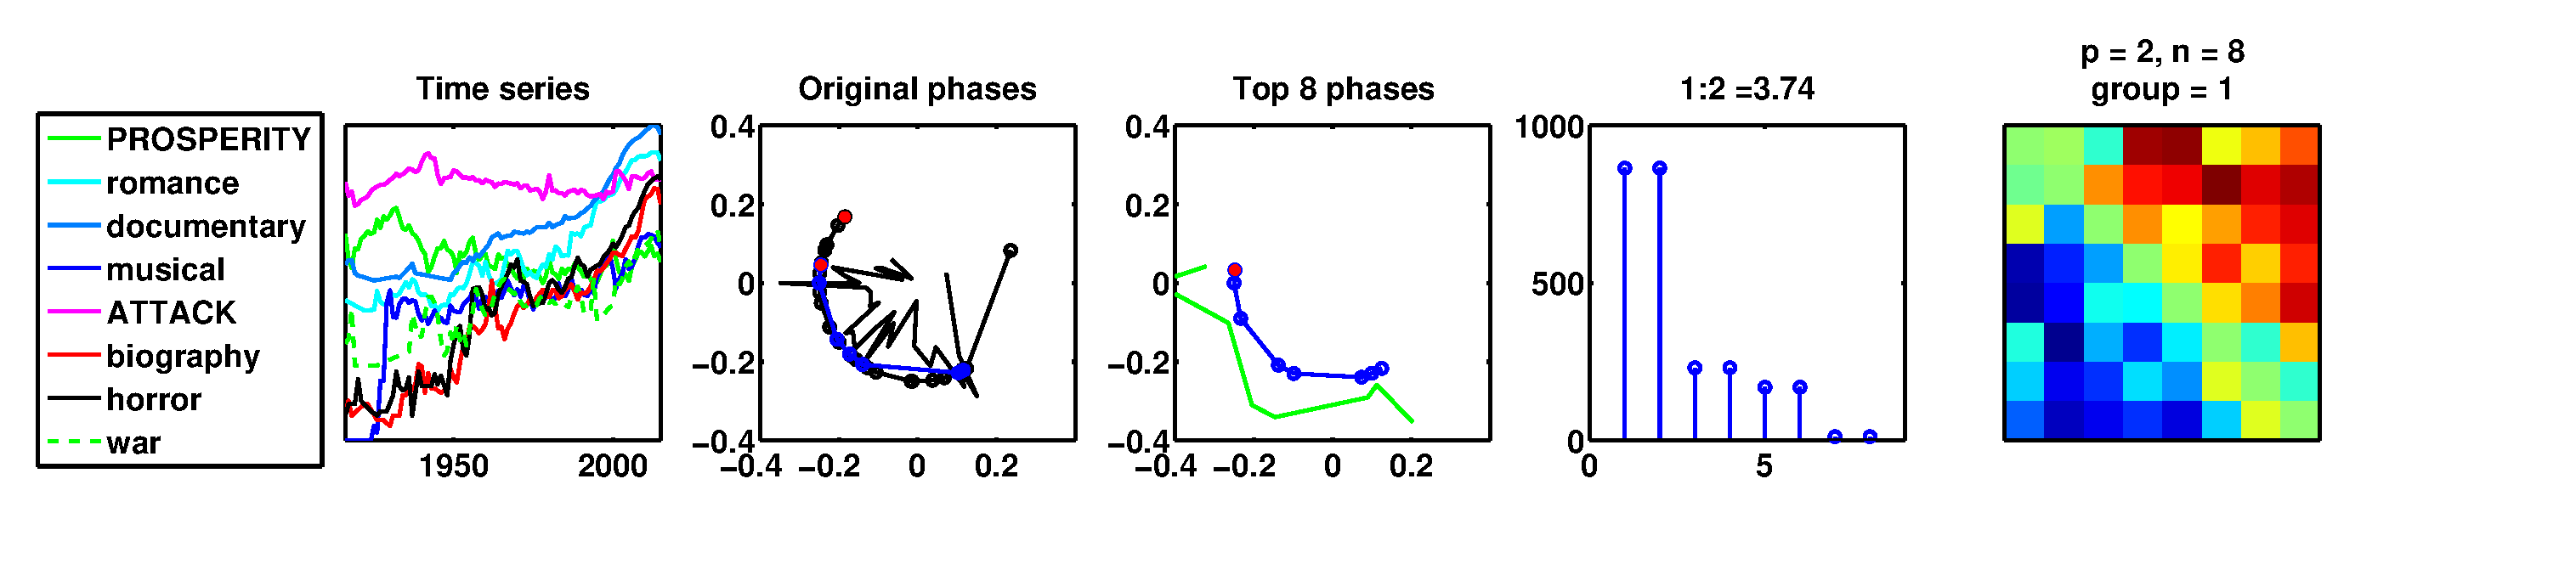
\includegraphics[trim = 0 0 130 0, clip, width=\textwidth]{pictures/_p2_n8_gp1.eps}
\caption{Results with n=8.}
\end{figure}

\begin{figure}[H]
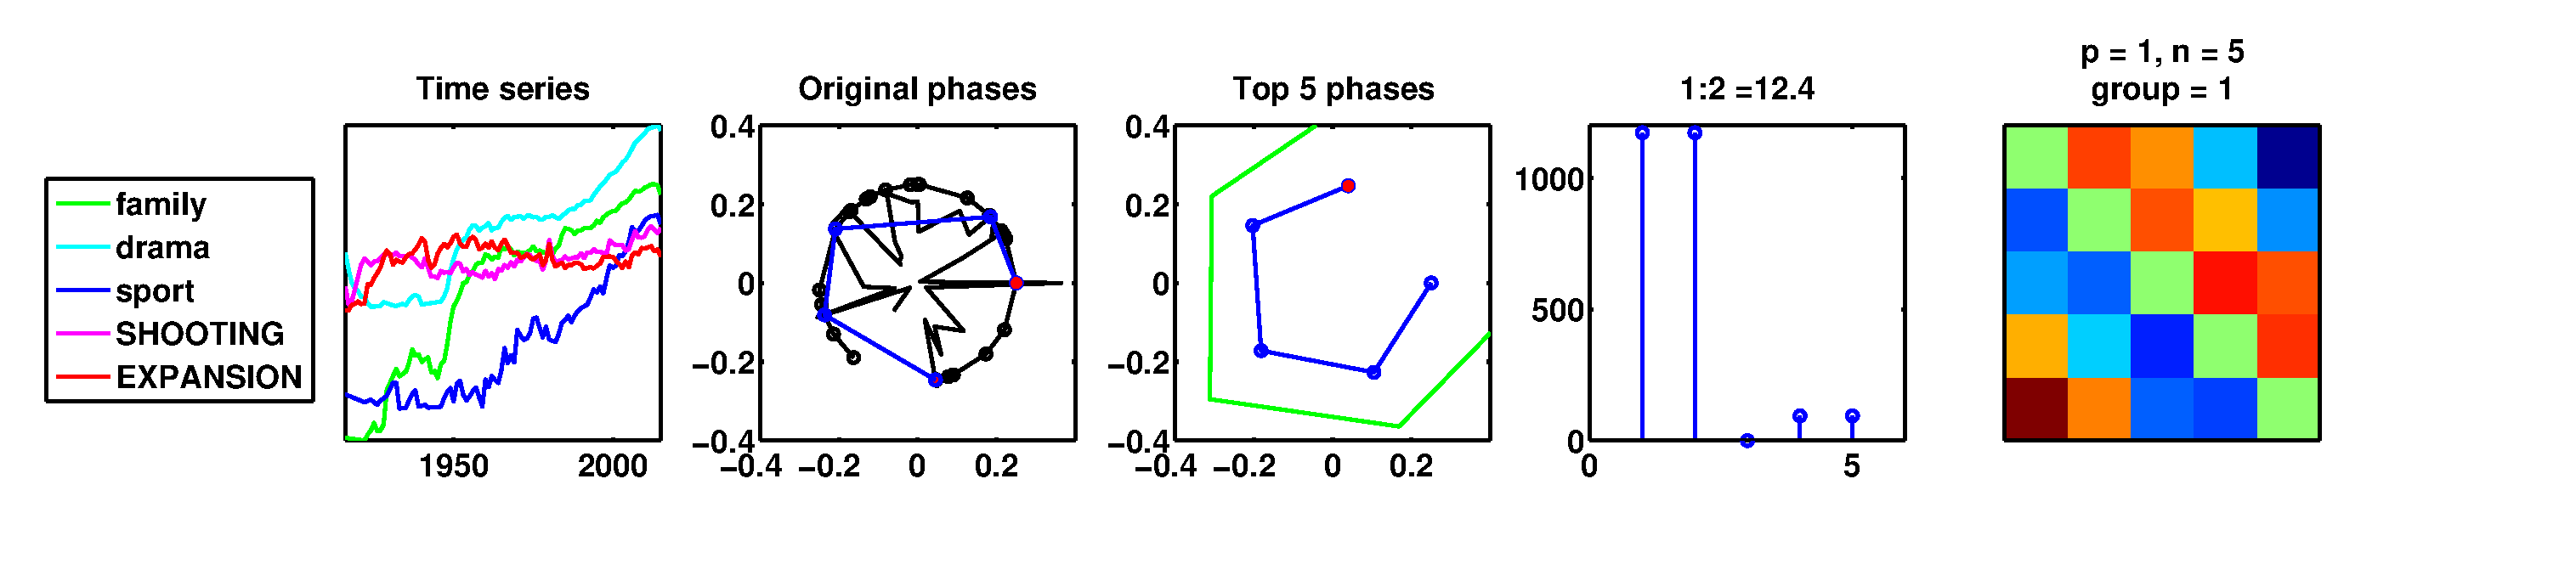
\includegraphics[trim = 0 0 130 0, clip, width=\textwidth]{pictures/_p1_n5_gp1.eps}
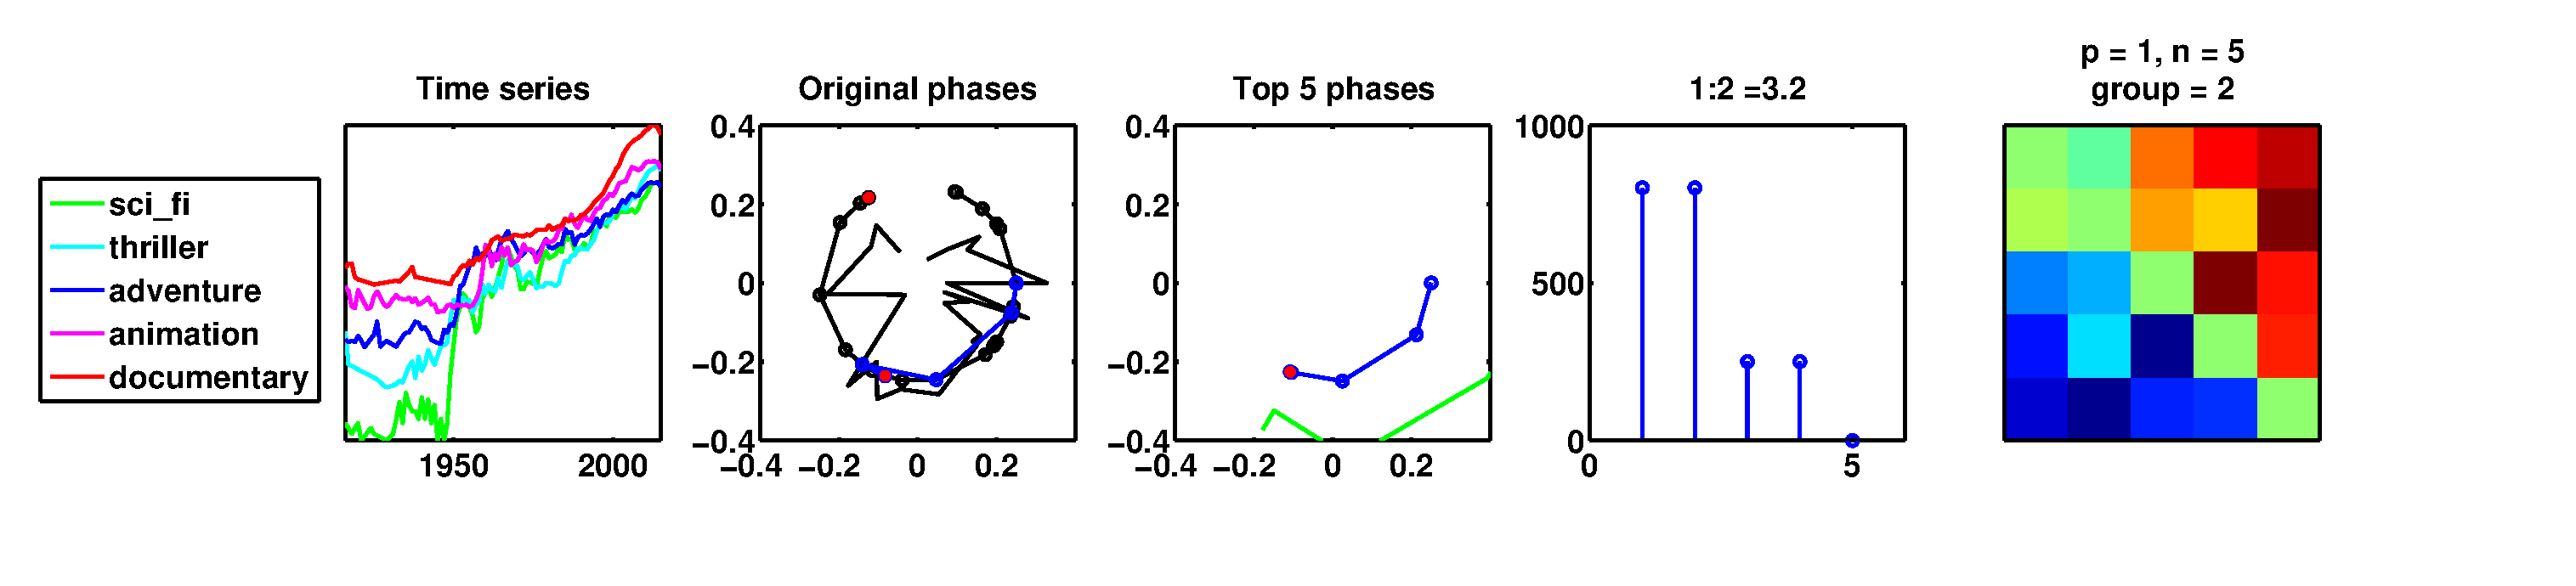
\includegraphics[trim = 0 0 130 0, clip, width=\textwidth]{pictures/_p1_n5_gp2.eps}
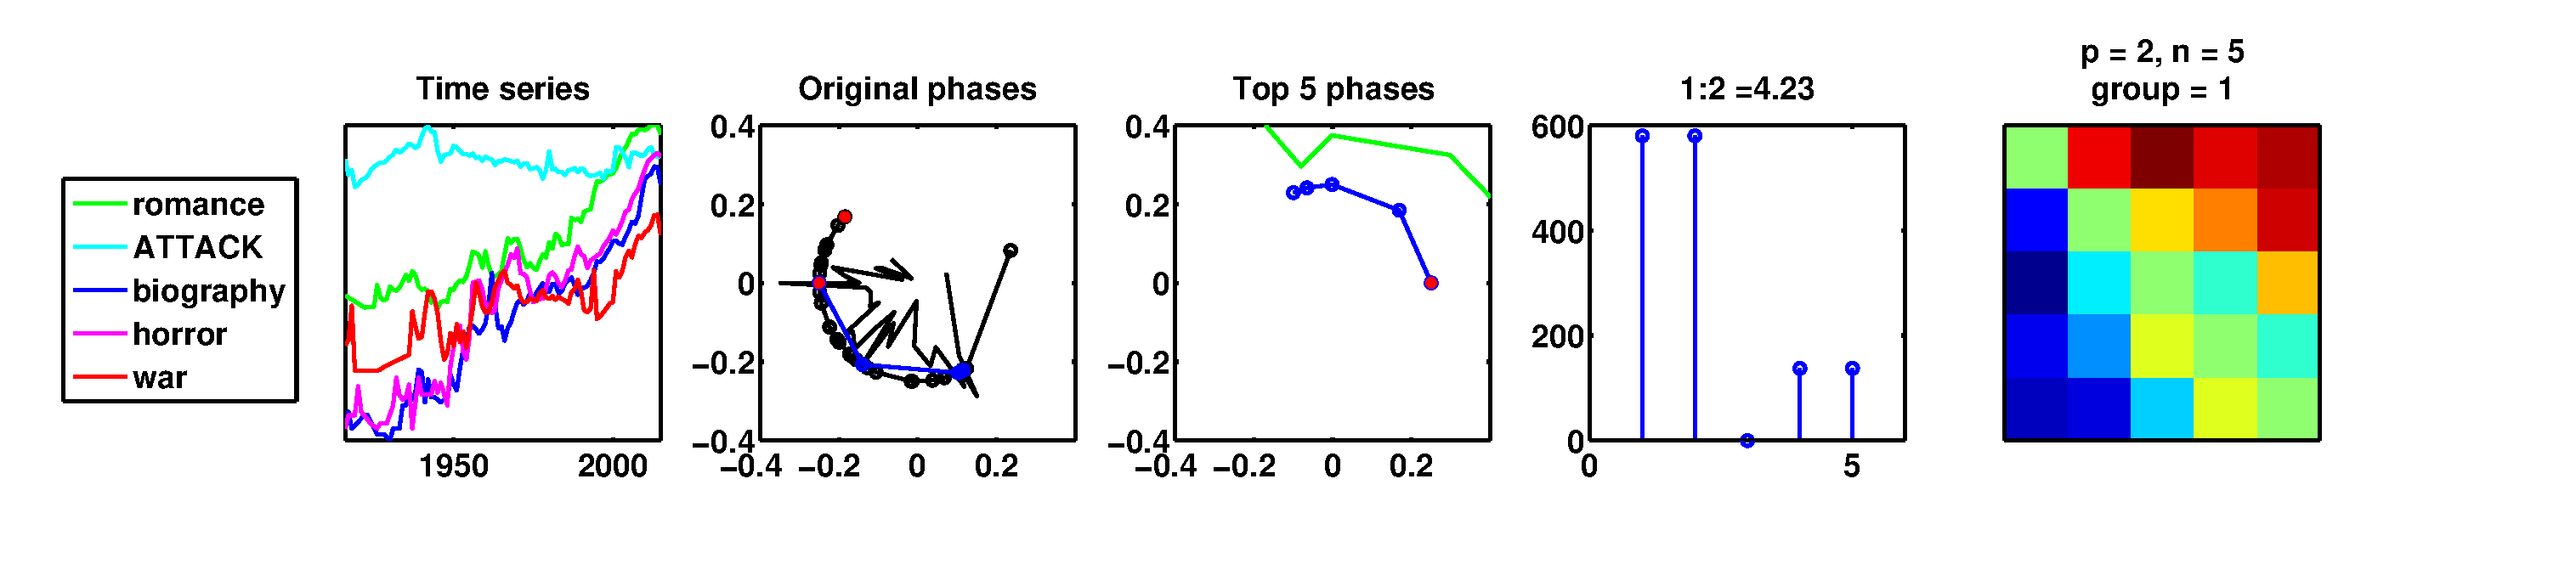
\includegraphics[trim = 0 0 130 0, clip, width=\textwidth]{pictures/_p2_n5_gp1.eps}
\caption{Results with n=5.}
\end{figure}

In each figure, the first subplot on the left shows the original traces (log scale) of the $n$ categories. The next subplot shows the original phase plot in black with the final $n$ categories highlighted in blue with the new ordering. Mostly the ordering from the initial analysis is preserved, but there are a few places (\verb|p=1|, \verb|n=5|, \verb|group=2|, for example) where if two categories were initially close together, they get exchanged in the final ordering. The final three plots are the same thing that we have been looking at all along for the subset of $n$ categories. Note that for the eigenvector ratio label on subplot 4, I the label says 1:2, which is actually 1:3 since the eigenvalues are complex conjugates so 1 and 2 have the same absolute value. If the third eigenvector was equal to 0 (odd man out), then I took the ratio of the first to the next non-zero (first:fourth technically).

\subsection{Impressions}
\begin{itemize}
\item I like the set of five. It is easy to digest and has high e1:e2 ratios. Until I have some reason to do otherwise,  I'll look at sets of 5.
\item Group 2 is not fantastic. Of the three analyses shown, it has the lowest e1:e2 ratio. I will probably run it anyway when we look at the brain permutations.
\item I would like to cut off the first 40 years as before and see what those trends look like.
\end{itemize}

\section{2/6/16}
\subsection{Recent movie data (1955-2015)}
As before, I reduced the movie data to only more recent trends. I learned today that "talkies" started in the 1920's with the first feature length film with synchronized dialogue was released in 1927. This probably explains the leap in production of music and musical films in the late 1920's. It is interesting, however, that in analyzing only more recent trends, 
\begin{itemize}
\item Clusters become quite obvious by looking at the lead matrix;
\item First eigenvalue, group 1 analysis does not wrap around the full cycle anymore;
\item Second eigenvalue ordering has lower e1:e2 ratio with a fuzzier lead matrix and now wraps around a full cycle.
\end{itemize}

Observe the following results on only the recent data.

\begin{figure}[H]
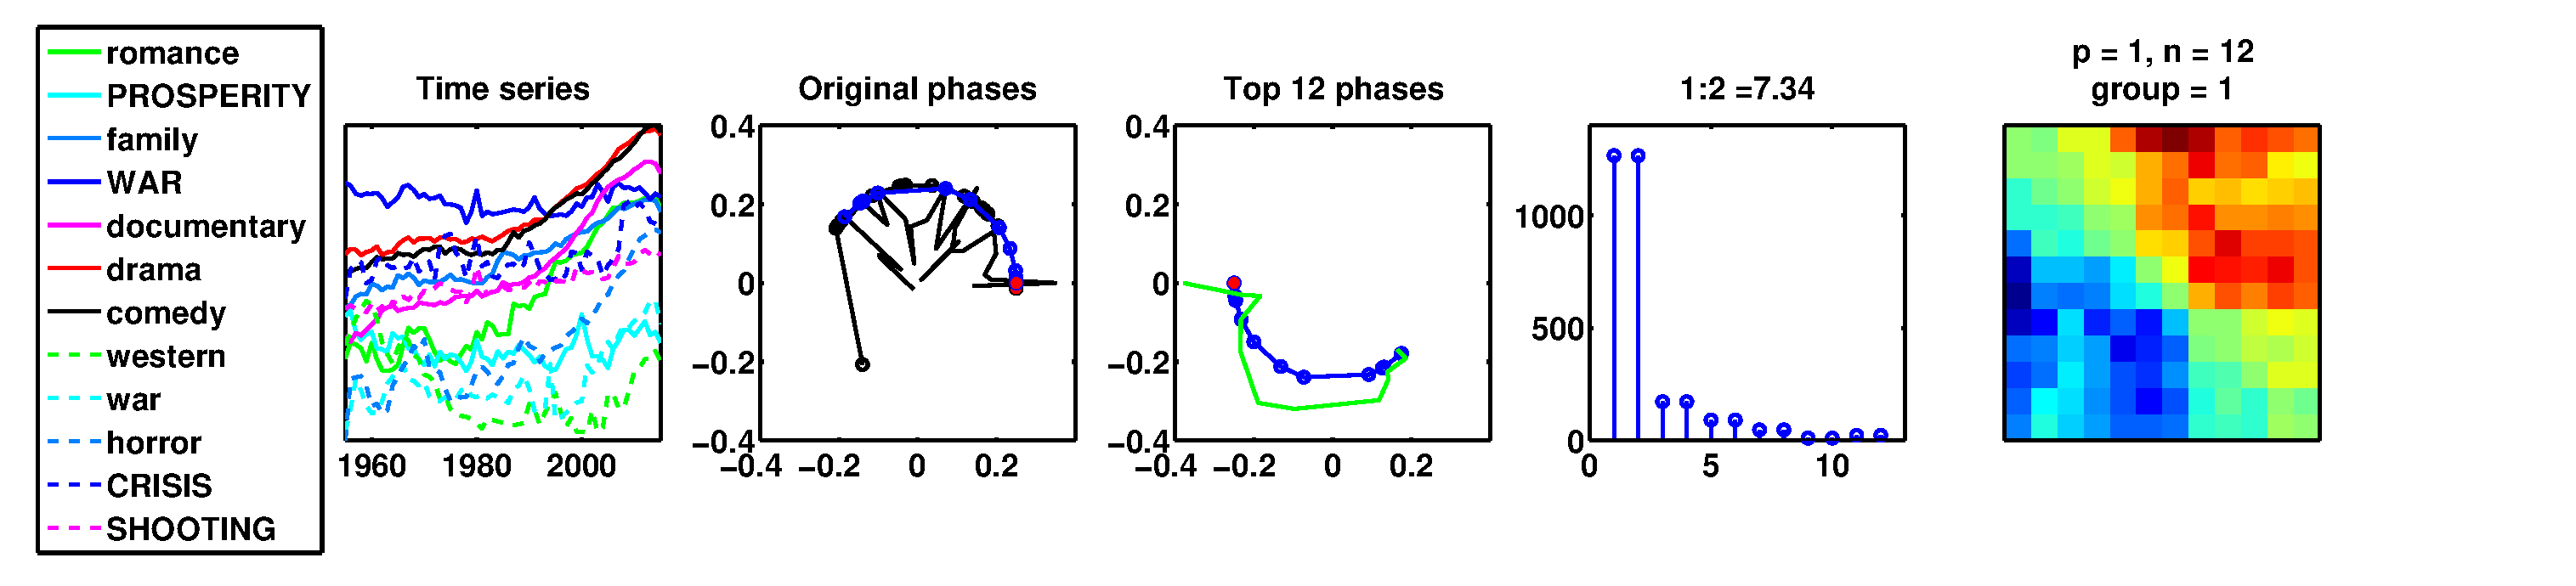
\includegraphics[trim = 0 0 130 0, clip, width=\textwidth]{pictures/movie_word_data_1955-2015_p1_n12_gp1.eps}
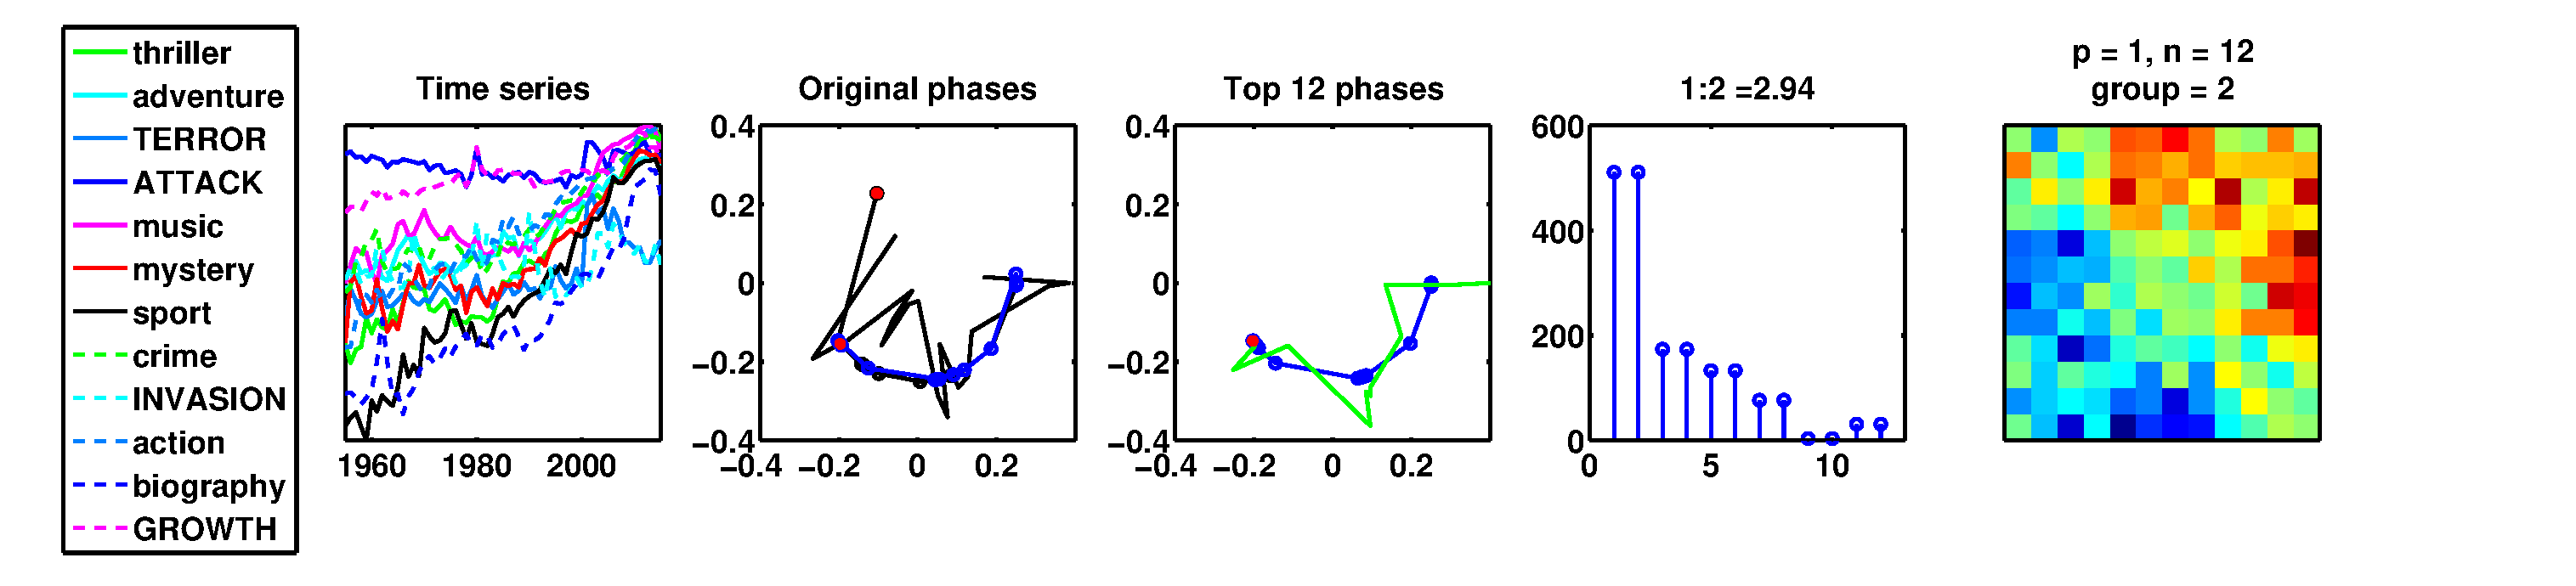
\includegraphics[trim = 0 0 130 0, clip, width=\textwidth]{pictures/movie_word_data_1955-2015_p1_n12_gp2.eps}
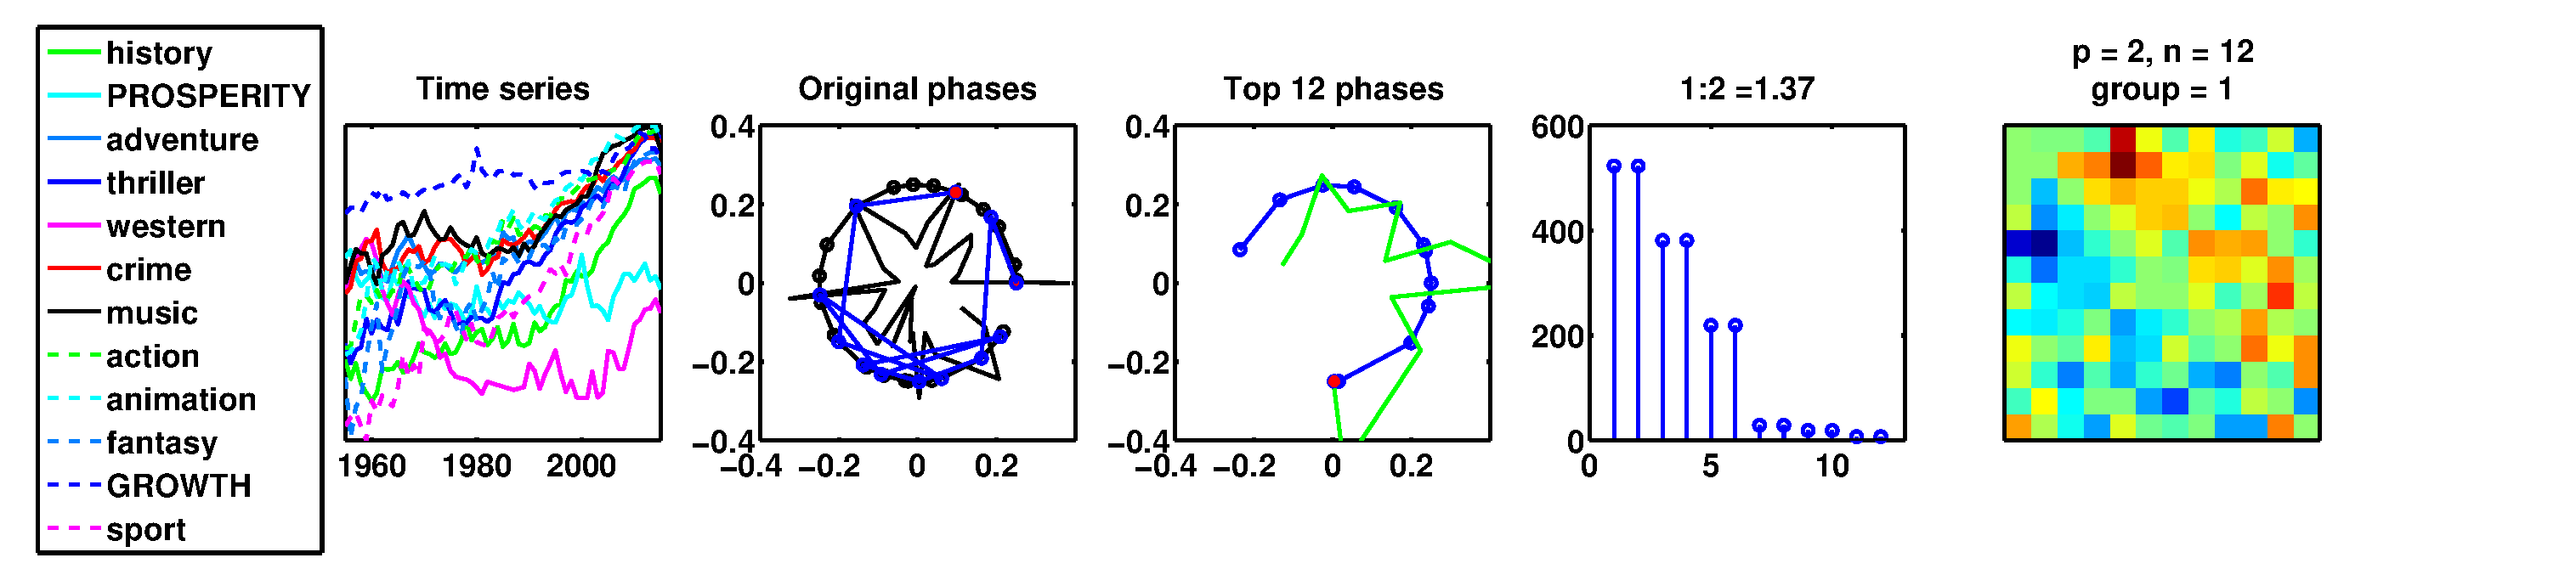
\includegraphics[trim = 0 0 130 0, clip, width=\textwidth]{pictures/movie_word_data_1955-2015_p2_n12_gp1.eps}
\caption{Results with n=12.}
\end{figure}

\begin{figure}[H]
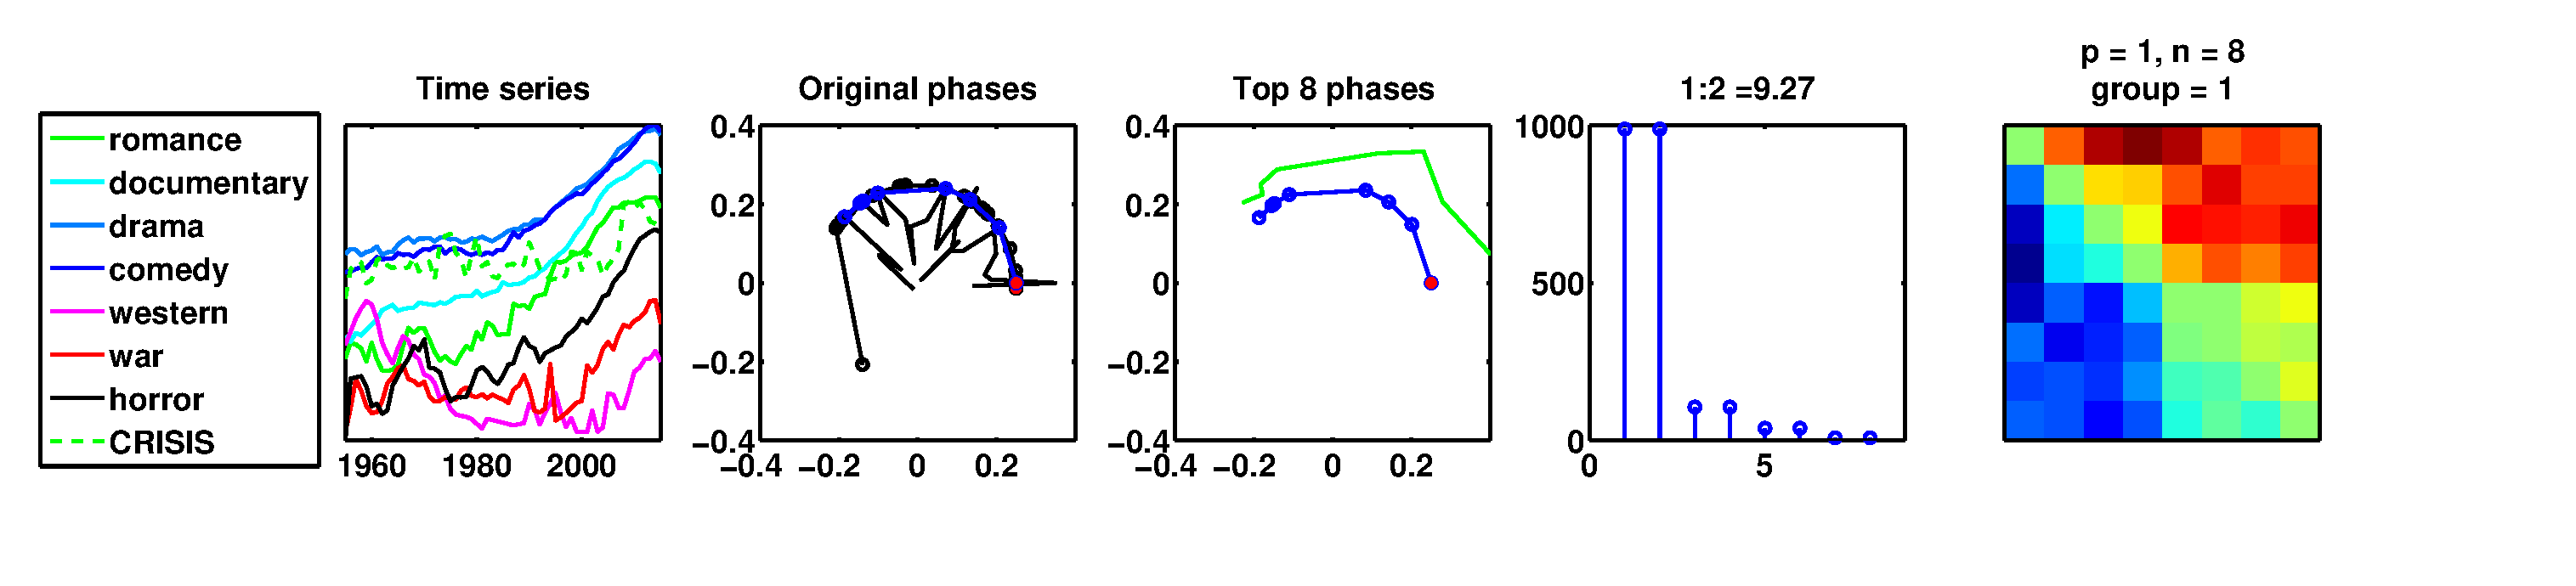
\includegraphics[trim = 0 0 130 0, clip, width=\textwidth]{pictures/movie_word_data_1955-2015_p1_n8_gp1.eps}
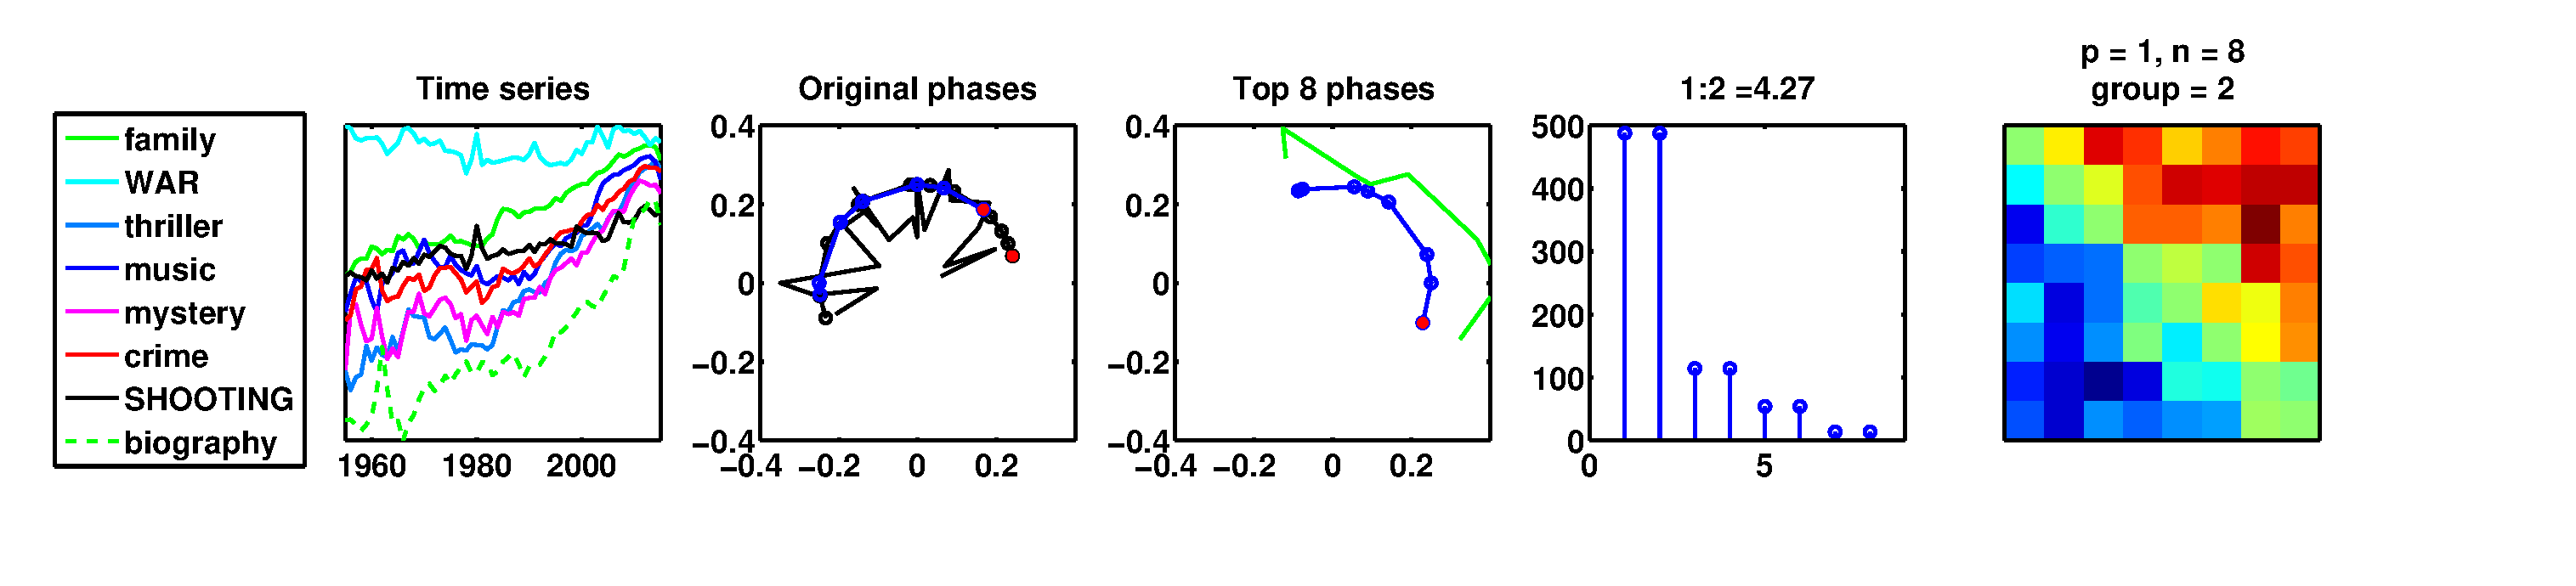
\includegraphics[trim = 0 0 130 0, clip, width=\textwidth]{pictures/movie_word_data_1955-2015_p1_n8_gp2.eps}
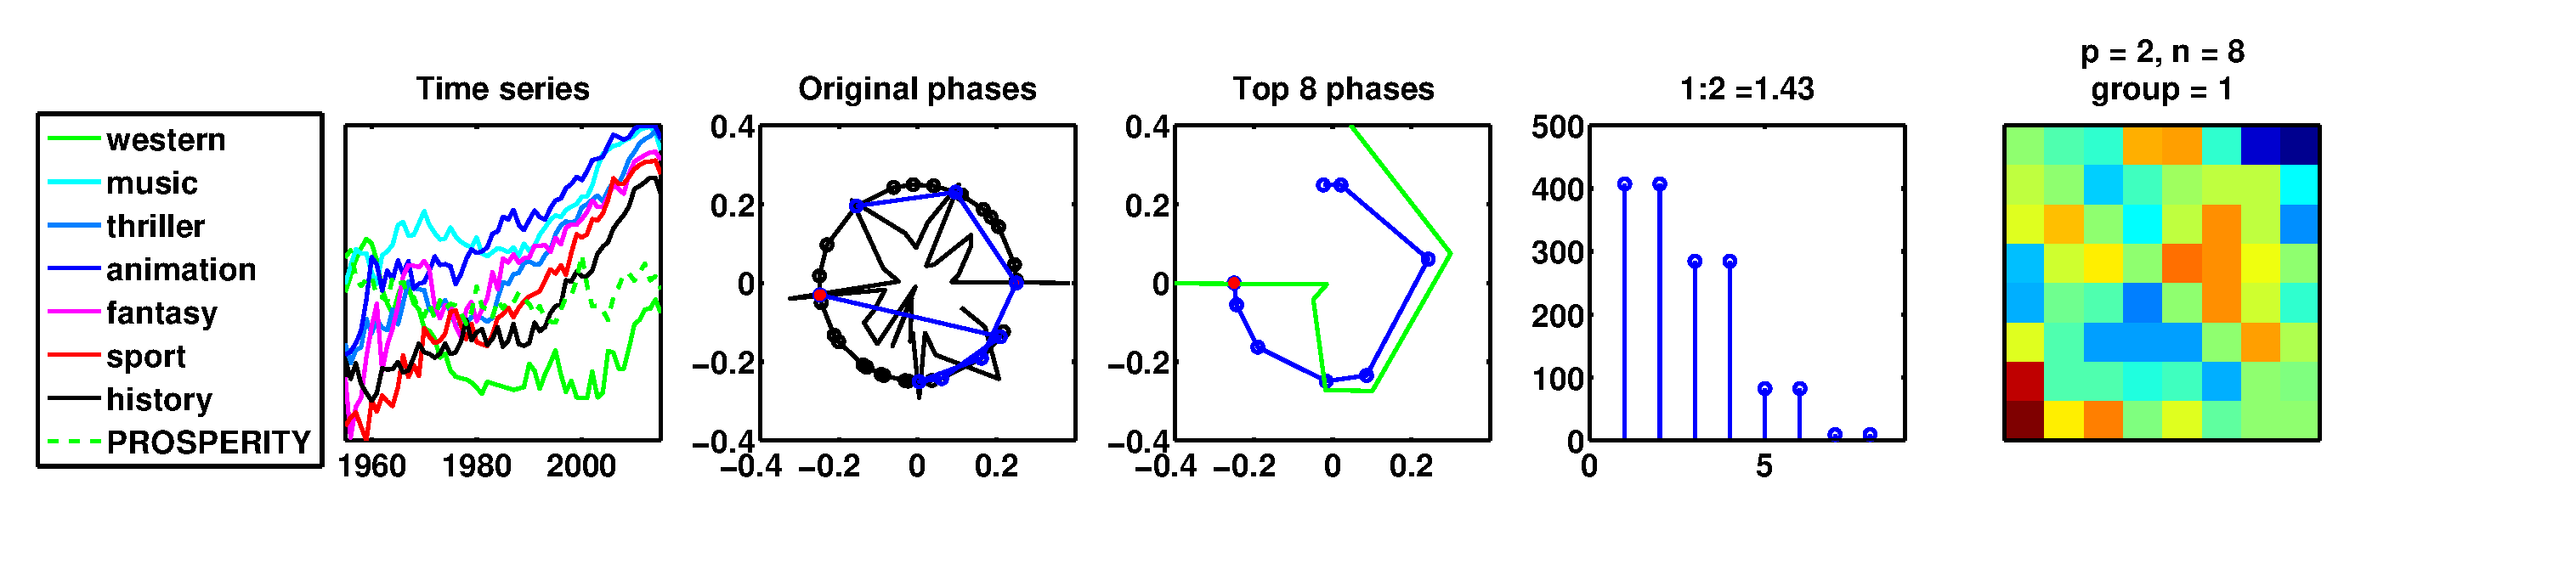
\includegraphics[trim = 0 0 130 0, clip, width=\textwidth]{pictures/movie_word_data_1955-2015_p2_n8_gp1.eps}
\caption{Results with n=12.}
\end{figure}

\begin{figure}[H]
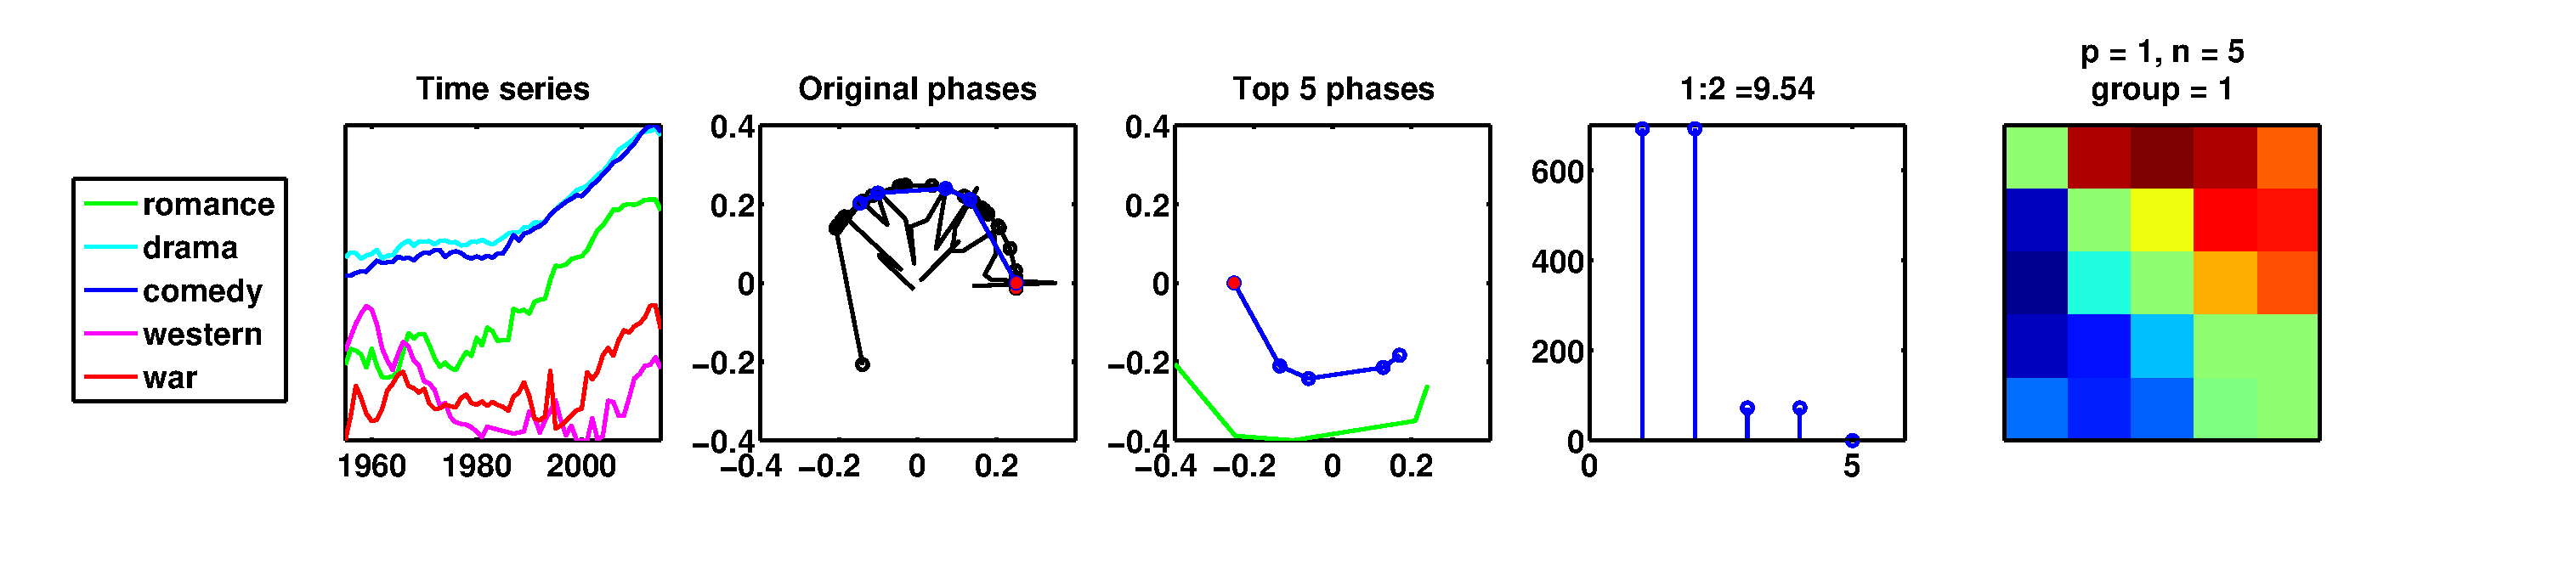
\includegraphics[trim = 0 0 130 0, clip, width=\textwidth]{pictures/movie_word_data_1955-2015_p1_n5_gp1.eps}
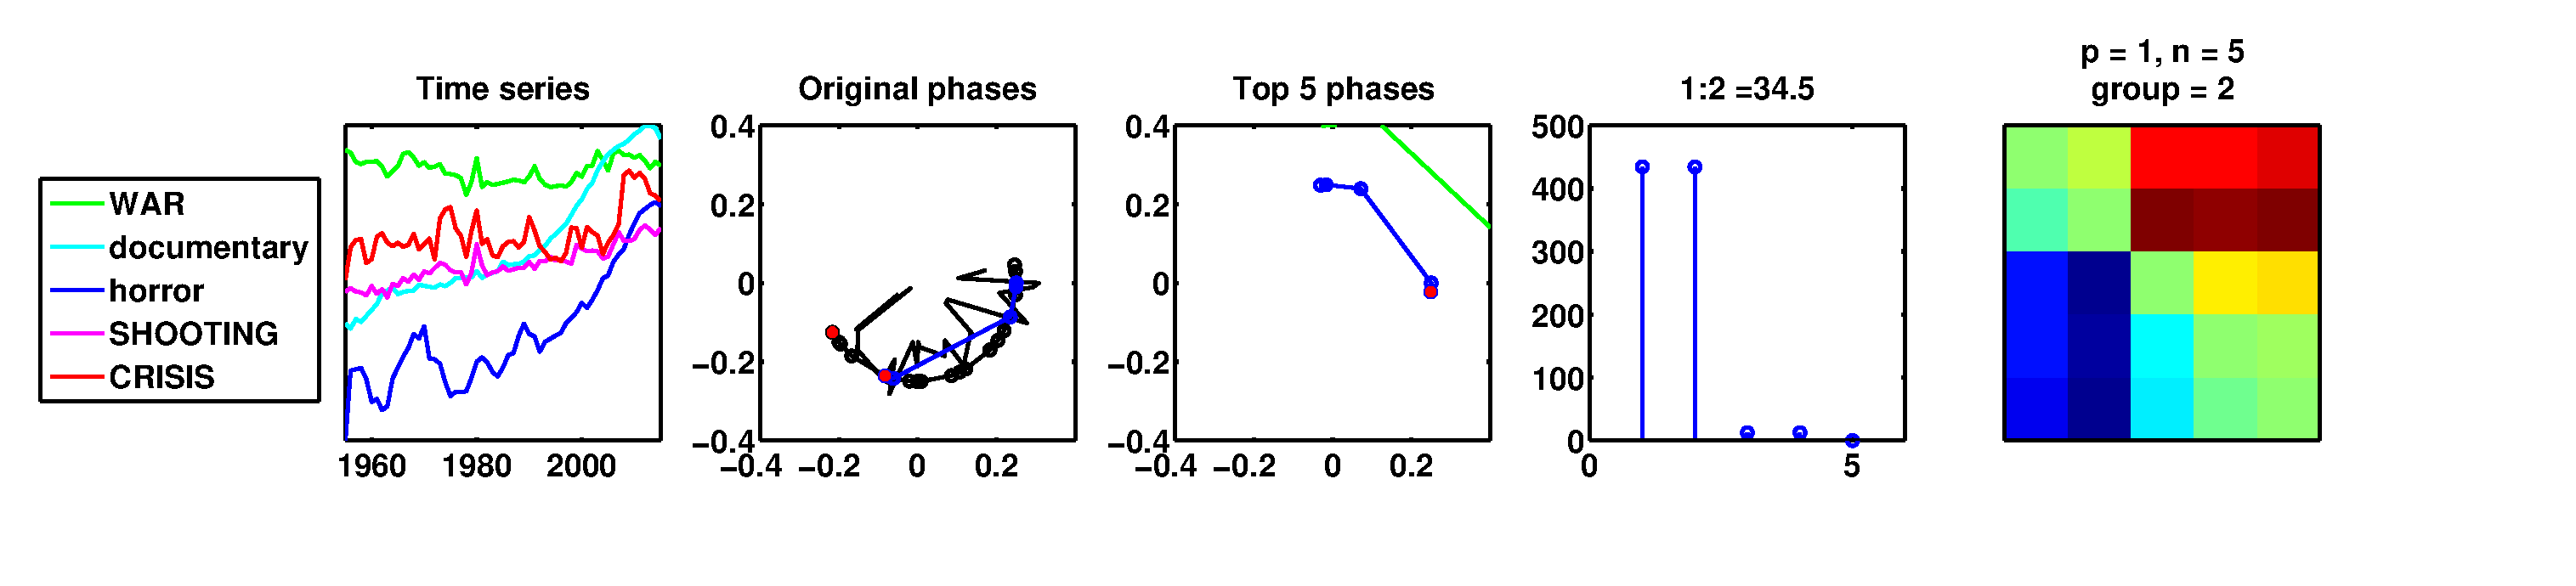
\includegraphics[trim = 0 0 130 0, clip, width=\textwidth]{pictures/movie_word_data_1955-2015_p1_n5_gp2.eps}
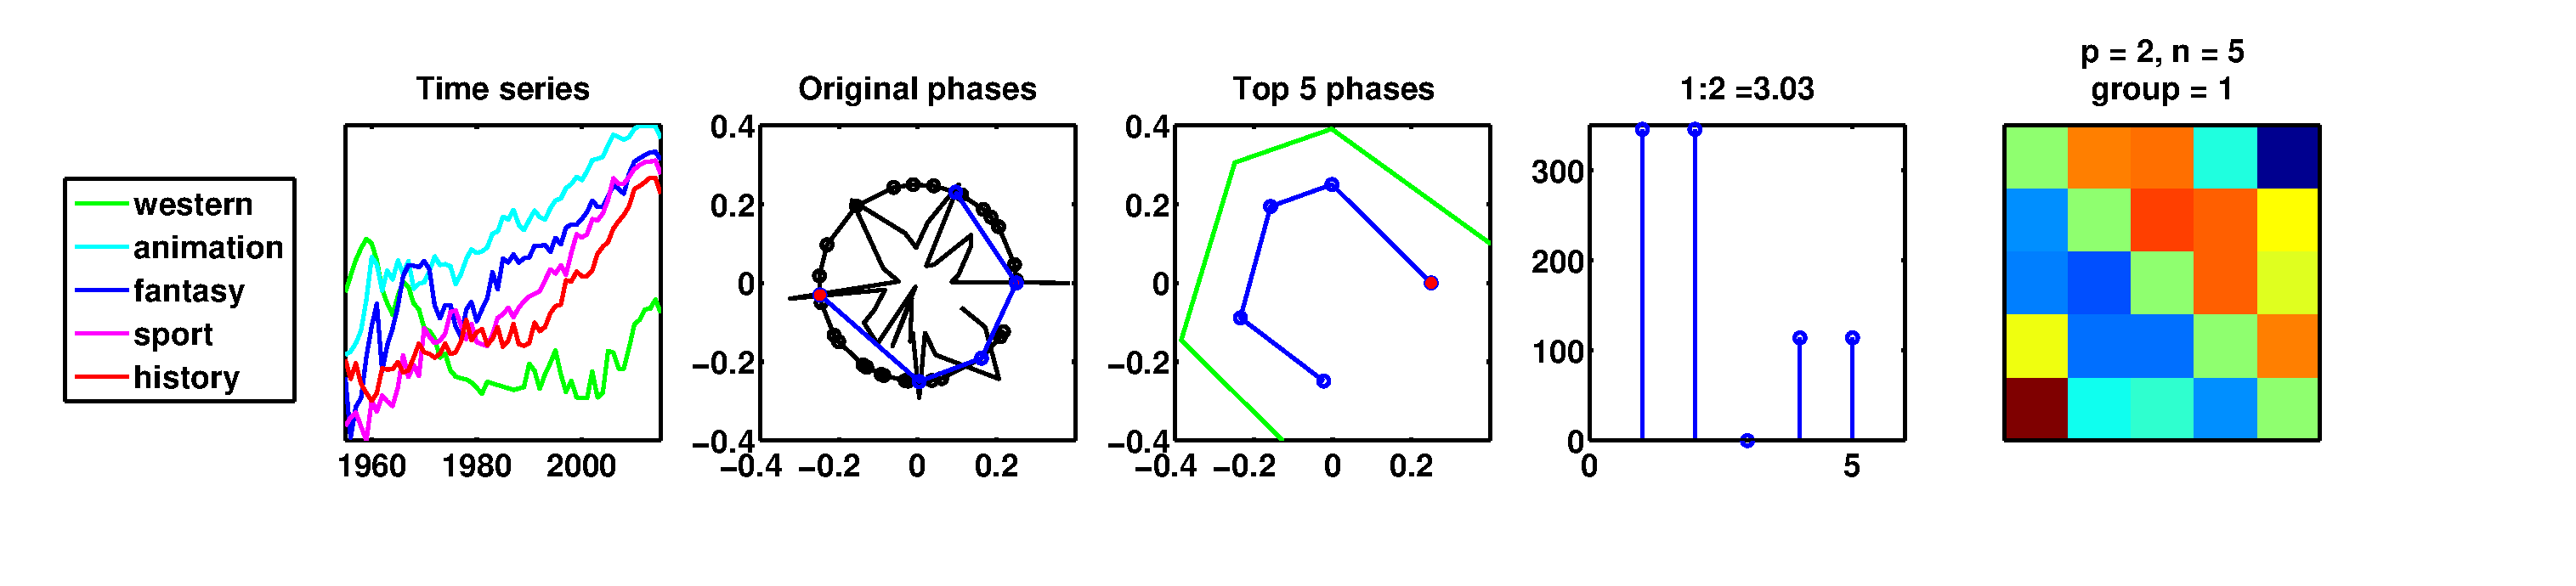
\includegraphics[trim = 0 0 130 0, clip, width=\textwidth]{pictures/movie_word_data_1955-2015_p2_n5_gp1.eps}
\caption{Results with n=12.}
\end{figure}


\end{document}